% Retoca las líneas marcadas con TODO según las necesidades

\documentclass[oneside,a4paper,12pt]{book} % TODO: cambia "oneside" por "twoside" a la hora de imprimirlo

\usepackage[spanish]{babel}
\usepackage[utf8]{inputenc}
\usepackage{geometry}
\usepackage{makeidx}
\usepackage{url}
\usepackage{graphicx}
\usepackage{color}
\usepackage{caption}
\usepackage{acronym}
\usepackage{hyphenat}
\usepackage{a4wide}
\usepackage[normalsize]{subfigure}
\usepackage{float}
\usepackage{titlesec}
\usepackage[Lenny]{fncychap}
\usepackage{listings} % para poder hacer uso de "listings" propios (p.ej. códigos)
\usepackage{eurosym} % para poder usar el símbolo del euro con \euro {xx}
\usepackage{hyperref} % TODO: añade la opción hidelinks para imprimirlo (los enlaces no aparecerán resaltados)
\usepackage{pdflscape}
\usepackage{multirow}
\usepackage[table,xcdraw]{xcolor}
\usepackage{fancyhdr}
\usepackage{longtable}
\usepackage[newfloat]{minted}
\usepackage{caption}
\usepackage{tikz-uml}
\usepackage{amsmath}
\usepackage{amssymb}
\usepackage{wrapfig}

%Fancyhdr Styles
\fancypagestyle{frontmatter}{%
    \fancyhf{} % clear all fields
    \renewcommand{\headrulewidth}{0pt}
    \lhead{}
    \lfoot[\thepage]{}
    \rfoot[]{\thepage} 
    }%
\fancypagestyle{mainmatter}{%
    \fancyhf{} % clear all fields
    \renewcommand{\headrulewidth}{0.5pt}
    \renewcommand{\footrulewidth}{0pt}
    \lhead[\leftmark]{Daniel García Estévez}
    \rhead[Daniel García Estévez]{\rightmark}
    \lfoot[\thepage]{}
    \rfoot[]{\thepage} 
}%

\setminted[]{
xleftmargin=.75cm,
xrightmargin=.75cm,
frame=single,
framesep=.25cm,
linenos,
tabsize=2,
breaklines
}

% Para que no parta las palabras
\pretolerance=10000
\renewcommand{\lstlistingname}{Algorithm}% Listing -> Algorithm
\renewcommand{\lstlistlistingname}{List of \lstlistingname s}% List of Listings -> List of Algorithms
\newcommand{\bigrule}{\titlerule[0.5mm]} \titleformat{\chapter}[display] % cambiamos el formato de los capítulos
{\bfseries\Huge} % por defecto se usaron caracteres de tamaño huge en negrita
{% contenido de la etiqueta 
\titlerule % línea horizontal 
\filright % texto alineado a la derecha 
\Large\chaptertitlename\ % capítulo e índice en tamaño large
\Large % en lugar de 
\Huge \Large\thechapter} 
{0mm} % espacio mínimo entre etiqueta y cuerpo
{\filright} % texto del cuerpo alineado a la derecha
[\vspace{0.5mm} \bigrule] % después del cuerpo, dejar espacio vertical y trazar línea horizontal gruesa
\geometry{a4paper, left=3.5cm, right=2cm, top=3cm, bottom=2cm, headsep=1.5cm}

\newenvironment{code}{\captionsetup[code]{type=listing}}{}
\SetupFloatingEnvironment{listing}{name=Código}

% Definición de mis propios tipos: Códigos, Ecuaciones y Tablas
\DeclareCaptionType{myequation}[Ecuación][Índice de ecuaciones]
\DeclareCaptionType{mycode}[Código][Índice de Códigos]

\hyphenation{fuer-tes}
\hyphenation{mul-ti-ca-pa}
\hyphenation{res-pues-ta}
\hyphenation{di-fe-ren-tes}
\hyphenation{de-sa-rro-lla-dos}
\hyphenation{re-pre-sen-tan-do}

 % archivo de configuracin de estilo

\makeindex

\begin{document}
\baselineskip 1.\baselineskip

\pagestyle{frontmatter}
\frontmatter
\thispagestyle{empty}

\begin{figure}[htb]
  \centerline{\resizebox{\textwidth}{!}{
\includegraphics{figuras/logo_upc}}}
\end{figure}

\begin{center}
  \vspace{2cm}
  {\Large {\bf INGENIERÍA INVERSA ASISTIDA POR INTELIGENCIA ARTIFICIAL}}
 
  \vspace{6cm}
  {\large {\bf DANIEL GARCÍA ESTÉVEZ}}
  
  \vfill
  {\bf Director/a}: ALEX PAJUELO GONZALEZ (Departamento de Arquitectura de Computadores) \\
  {\bf Codirector/a}: JUAN JOSÉ COSTA PRATS (Departamento de Arquitectura de Computadores) \\
  {\bf Titulación}: Grado en Ingeniería Informática (Tecnologías de la información) \\
  \vspace{0.5cm}
  {\bf Memoria del trabajo de fin de grado} \\
  {\bf Facultat d'Informàtica de Barcelona (FIB)} \\
  {\bf Universitat Politècnica de Catalunya (UPC) - BarcelonaTech} \\

\end{center}


\clearpage\hbox{}\thispagestyle{empty}\newpage

% \cleardoublepage
\chapter*{Resumen\markboth{Resumen}{Resumen}}


\cleardoublepage

\tableofcontents

\listoffigures

% \listoflistings

\listofmyequations

\listoftables

\cleardoublepage % aqui se cargan todas las "primeras paginas"

% Bibliografa
\let\OLDthebibliography=\thebibliography
\def\thebibliography#1{\OLDthebibliography{#1}
  \addcontentsline{toc}{chapter}{\bibname}}

\mainmatter
\pagestyle{mainmatter}
\setcounter{page}{1}

\chapter{Introducción}
\label{cap:introducion}

\setcounter{page}{1}

\begin{flushright}
    \begin{minipage}[]{10cm}
        \emph{Basically, if reverse engineering is banned, then a lot of the open source community is doomed to fail}\\
    \end{minipage}\\

    Jon Lech Johansen, \textit{}\\
\end{flushright}

\vspace{1cm}

Antes de entrar en profundidad en el proyecto que en esta memoria se detalla me gustaria introducir formalmente el concepto de ``ingeniería inversa'' o conocida en el mundo de la
informatica como \textit{reverse engineering}. La ingineria inversa es el proceso de extraer conocimiento o el diseño por cualquier cosa que el humano haya hecho. Por lo tanto,
no es un concepto que solo acotemos dentro de la ingineria informatica si no que se puede aplicar a cualquier proceso ingineril. De hecho, este proceso es bastante similar al
metodo cientifico, con la unica diferencia que la ingineria inversa solo se aplica sobre cosas que ha hecho un humano y en el metodo cientifico lo aplicamos en fenomenos
naturales.

La ingineria inversa es usada normalmente para obtener conocimiendo desconocido o la filosofia del diseño cuando esta información no esta disponible, ya sea porque su propietario
ha decidido no compartirla o porque esta información esta perdida o destruida. \cite{alma991003132729706711}

La ingienería inversa aplicada al \textit{software} es el mismo concepto pero aplicada a programa en su formato binario, con el objetivo de obtener el codigo fuente en un lenguaje
de programación concreto y así poder obtener información como el diseño del programa. De hecho, la ingeniería inversa aplicada al \textit{software} requiere diferentes artes:
descifrado de codigos, resolución de puzzles, programación y analisis logico.

Las aplicaciones de la ingineria inversa son muy variadas, pero podemos destacar dos categorias: seguridad y desarrollo de \textit{software}.

Sus aplicaciones en seguridad son muy variadas, pero normalmente se le relaciona con \textit{malware}, algoritmos criptograficos y auditorias sobre binarios.

Dentro del mundo del \textit{software} malicioso vemos que la ingeniería inversa se utiliza en dos aspectos diferentes. Desde el punto de perspectiva de los que desarrollan
\textit{software} malicioso utilizan la ingeniería inversa para poder encontrar vulnerabilidades en los programas que quieren infectar. En canvio, desde el punto de vista de los 
desarrolladores de antivirus, utilizan la ingeniería inversa para poder diseccionar y analizar cada programa malicioso.

Tambien se puede aplicar ingeniería inversa sobre algoritmos criptograficos de tal manera que podamos averiguar que tan seguro es ese mensage encriptado, o incluso en caso de utilizar
algoritmos basados en llaves, en los cuales la especificación del algoritmo de encriptación es conocico pero que cada implementación especifica puede variar, encontrar vulnerabilidades
en estos algoritmos.

Y por ultimo, tambien la ingineria inversa se aplica para realizar auditorias sobre binarios, de tal manera que podamos detectar si un programa es seguro o no, encontrar sus vulnerabilidades
para poder corregirlas. Por lo tanto, cuanto mejores sean las herramientas de ingineria inversa que se apliquen podremos encontrar con mucha mas eficacia problemas de seguridad en 
\textit{software} propietario.

Como he mencionado con anterioridad, la ingeniería inversa tambien se aplica dentro del desarrolo de \textit{software}, estas aplicaciones las podemos encontrar en diferentes etapas
por ejemplo cuando disponemos de un \textit{software} propietario y a documentación es escasa, el uso de herramientas de ingineria inversa nos podrian ayudar a conseguir mas interoperabilidad
con el \textit{software} propietario.

Otras de las aplicaciones, y que he mencionado anteriormente, es el comprobar la robustez y calidad de un programa informatico, de tal manera que se pueda corregir posibles problemas
de seguridad o problemas funcionales.

Una vez introducido el concepto de ingeniería inversa de manera general, creo que es interesante contestar a la siguiente pregunta: \textbf{¿Es la ingeniería inversa legal?}

Como hemos podido ver en los parrafos anteriores, muchas veces aplicamos ingeniería inversa sobre un \textit{software} propietario, algunos con fines de conocer vulnerabilidades y corregirlas
y otros con fines de encontrar estas vulnerabilidades para tener un punto de ataque. En otras palabras, la legalidad de la aplicacion de ingineria inversa dependera mucho de para
que lo estamos aplicando, la finalidad, y sobre que lo estamos aplicando.

En conclusión, la ingeniería inversa es un proceso complejo y que requiere de muchas habilidades y que sus aplicaciones son muy variadas, desde auditorias sobre binarios hasta mejorar 
la interoperabilidad de dos programas. 

\section{Contextualización}
\label{sec:contextualizacion}

% Corregido

Como bien he mencionado con anterioridad, este proyecto se enmarca dentro de un proyecto de final de Grado de Ingeniería Informática, en la especialidad de Tecnologías de la Información.
Este grado se imparte en la Facultad de Informática de Barcelona (FIB) y está dentro del contexto de la Universitat Politècnica de Catalunya (UPC).

En este trabajo se ha propuesto abordar una serie de competencias técnicas, que pasaré a detallar más adelante, que están estrechamente relacionadas con la especialidad cursada. Estas
son las competencias técnicas:

\begin{itemize}
    \item \textbf{CTI3.3} Diseñar, implantar y configurar redes y servicios.
    \item \textbf{CTI3.4} Diseñar \textit{software} de comunicaciones.
\end{itemize}

\section{Identificación del problema}
\label{sec:problema}

Como he explicado en el capitulo \ref{cap:introducion} la ingeniería inversa es aplicada en una infinidad de campos y de los cuales hoy en dia es utilizada. Pero como he mencionado
aplicar ingeniería inversa no es una tarea facil, ya que actualmente los programas que podemos encontrar en el mercado son de tal complejidad que aplicar ingineria inversa sobre la
totalidad del programa supone horas y horas de trabajo, teniendo el riesgo de que los resultados obtenidos no se asemejen a la realidad.

Esta complejidad no solo viene dada por el gran tamaño de los programas actuales si no de las tecnicas que se utilizan para poder ocultar aún más el programa original. Algunas
de estas tecnicas son \textit{constant blinding}\footnote{Esta tecnica consiste en poner un valor aleatorio a las constantes (a traves de operaciones como la XOR)}, cambiar el 
encoding de las variables\footnote{Busca la ocultación del valor de la variable cambiando su representación de datos}, agregación de datos\footnote{Busca agrupar variables del mismo
tipo, por ejemplo bajo un \textit{struct}}, separación de datos\footnote{Al contrario que la agregación de datos, esta busca separar los datos en unidades mas pequeñas, por ejemplo
de un \textit{short} a un \textit{char}}, \textit{dead code insertion}\footnote{Agreagar codigo redundante al programa}, \textit{loop unrolling}\footnote{Es una tecnica que aplican
los compiladores que ademas de disminuir el coste computacional del programa hace que el codigo sea menos legible}, entre otras. \cite{TecnicasIlegibleBinario}

Tambien a la hora de aplicar ingineria inversa debemos sumar la complejidad de las aplicaciones distribuidas, es decir, antes cuando disponiamos de un programa disponiamos de su
codigo en su totalidad auqnue este fuese en forma de un binario. Con las aplicaciones distribuidas, el programa se ha segmentado en diferentes parte y estas partes cada una se
puede encontrar en una maquina diferente, probocando que no dispongamos aveces del todo el programa y por lo tanto, de todo su diseño y logica.

Por lo tanto, debido a las tecnicas de ocultación de codigo, las optimizaciones que el compilador puede aplicar sobre el codigo, el gran tamaño de los programas modernos y el auge
de las aplicaciones distribuidas hacen que la tarea de aplicar ingeniería inversa sobre un programa sea muy compleja y que las soluciones actuales, que detallare en la sección
\ref{sec:alternativas}, no son capaces de dar buenos resultados, si no que dan una especie de pseudocódigo que nos puede ayudar a entender la logica del programa.

Todos estos factores contribuyen a que aplicar ingienería inversa sea muy complejo y costoso, y por lo tanto inviable en muchos casos para ciertos escenarios.

\section{Terminología y definiciones}
\label{sec:terminalogia}

% Corregido

En este apartado pasaremos a detallar ciertos términos reiterativos que veremos a lo largo del proyecto y que son de especial importancia. Las definiciones son las siguientes:

\begin{itemize}
    \item \textbf{Large Lenguage Model:} un LLM o \textit{Large Lenguage Model} son modelos \textit{Pre-trained Lenguage Models}\footnote{El concepto de pre entrenamiento en un modelo
                                        de lenguaje está relacionado con el aprendizaje por transferencia. La idea del aprendizaje por transferencia es reutilizar los conocimientos
                                        aprendidos en una o varias tareas y aplicarlos a tareas nuevas.} (PLM) a los cuales se han aumentado o el tamaño del modelo en sí o los datos.
                                        Con este aumento se dieron cuenta de que había una notoria mejora en términos de \textit{performance} y de la capacidad de los modelos en hacer
                                        ciertas tareas. \cite{ZhaoWayneXin2023ASoL}
    \item \textbf{Fine-tuning:} es una técnica de entrenamiento que consiste en reutilizar un modelo predefinido y preentrenado, de tal manera que ajustamos ciertas capas de la
                                red neuronal para obtener mejores resultados para nuestra tarea en específico.
\end{itemize}

\section{Actores implicados}
\label{sec:actores}

% Corregido

A continuación se pasarán a detallar a los actores implicados en el trabajo. Estos actores pueden participar de manera activa o pasiva dentro del proyecto, pero tiene una relevancia
importante dentro de este mismo:

\begin{itemize}
    \item \textbf{Investigador:} Este proyecto consta de un único investigador, Daniel García Estevez. Este se encargará de hacer tareas tales como la investigación de modelos a utilizar, 
                                 metodos de \textit{fine-tuning}, entre otras.
    \item \textbf{Director y codirector:} El director del trabajo de final de grado Alex Pajuelo Gonzalez perteneciente al CRAAX\footnote{Centre de Recerca d'Arquitectures Avançades de Xarxes}
                                        y profesor asociado a la UPC. Será el encargado de dirigir y supervisar este proyecto. Así mismo, el codirector del proyecto, Juan José Costa Prats
                                        perteneciente al CRAAX, ara tareas similares al director.
    \item \textbf{Experto en Inteligencia Artificial:} este proyecto constará con un experto en inteligencia artificial que dará soporte en temas más específicos que se salen fuera del alcance de
                                                    este proyecto. El experto es Jordi Nin Guerrero profesor titular en el Departamento de Operaciones, Innovación y Data Sciences en ESADE.
    \item \textbf{Colaboradores:} también contaremos con la ayuda de Xavi Verdú, profesor asociado de la UPC e investigador senior de PhD.
\end{itemize}
\chapter{Estado del arte de la ingeniería inversa}
\label{cap:estadoDelArte}

% TODO:daniel: Corregir y revisar El estado del arte de la ingeniería inversa

Antes de entrar en profundidad en el proyecto que en esta memoria se detalla me
gustaría introducir formalmente el concepto de ''ingeniería inversa'' o conocida
en el mundo de la informática como \textit{reverse engineering}. La ingeniería
inversa es el proceso de extraer conocimiento o el diseño por cualquier cosa que 
el humano haya hecho. Por lo tanto, no es un concepto que solo acotemos dentro de
la ingeniería informática, sino que se puede aplicar a cualquier proceso ingenieril.
De hecho, este proceso es bastante similar al método científico, con la única diferencia
que la ingeniería inversa solo se aplica sobre cosas que ha hecho un humano y en el
método científico lo aplicamos en fenómenos naturales.

La ingeniería inversa es usada normalmente para obtener conocimiento desconocido o la
filosofía del diseño cuando esta información no está disponible, ya sea porque su
propietario ha decidido no compartirla o porque esta información está perdida o 
destruida. \cite{alma991003132729706711}

La ingeniería inversa aplicada al \textit{software} es el mismo concepto, pero aplicada
a programa en su formato binario, con el objetivo de obtener el código fuente en un
lenguaje de programación concreto y así poder obtener información como el diseño del
programa. De hecho, la ingeniería inversa aplicada al \textit{software} requiere
diferentes artes: descifrado de códigos, resolución de puzzles, programación y análisis
lógico.

Las aplicaciones de la ingeniería inversa son muy variadas, pero podemos destacar dos
categorías: seguridad y desarrollo de \textit{software}.

Sus aplicaciones en seguridad son muy variadas, pero normalmente se le relaciona con
\textit{malware}, algoritmos criptográficos y auditorias sobre binarios.

Dentro del mundo del \textit{software} malicioso vemos que la ingeniería inversa se
utiliza en dos aspectos diferentes. Desde el punto de perspectiva de los que desarrollan
\textit{software} malicioso utilizan la ingeniería inversa para poder encontrar
vulnerabilidades en los programas que quieren infectar. En cambio, desde el punto de vista
de los desarrolladores de antivirus, utilizan la ingeniería inversa para poder diseccionar
y analizar cada programa malicioso.

También se puede aplicar ingeniería inversa sobre algoritmos criptográficos, de tal manera
que podamos averiguar que tan seguro es ese mensaje encriptado, o incluso en caso de utilizar
algoritmos basados en llaves, en los cuales la especificación del algoritmo de encriptación
es conocido, pero que cada implementación específica puede variar, encontrar vulnerabilidades
en estos algoritmos.

Y por último, también la ingeniería inversa se aplica para realizar auditorias sobre binarios,
de tal manera que podamos detectar si un programa es seguro o no, encontrar sus vulnerabilidades
para poder corregirlas. Por lo tanto, cuanto mejores sean las herramientas de ingeniería inversa
que se apliquen, podremos encontrar con mucha más eficacia problemas de seguridad en \textit{software}
propietario.

Como he mencionado con anterioridad, la ingeniería inversa también se aplica dentro del desarrollo
de \textit{software}, estas aplicaciones las podemos encontrar en diferentes etapas por ejemplo
cuando disponemos de un \textit{software} propietario y a documentación es escasa, el uso de
herramientas de ingeniería inversa nos podrían ayudar a conseguir más interoperabilidad con
el \textit{software} propietario.

Otras de las aplicaciones, y que he mencionado anteriormente, es el comprobar la robustez y calidad
de un programa informático, de tal manera que se pueda corregir posibles problemas de seguridad o
problemas funcionales.

Una vez introducido el concepto de ingeniería inversa de manera general, creo que es interesante
contestar a la siguiente pregunta: \textbf{¿Es la ingeniería inversa legal?}

Como hemos podido ver en los párrafos anteriores, muchas veces aplicamos ingeniería inversa sobre
un \textit{software} propietario, algunos con fines de conocer vulnerabilidades y corregirlas
y otros con fines de encontrar estas vulnerabilidades para tener un punto de ataque. En
otras palabras, la legalidad de la aplicación de ingeniería inversa dependerá mucho
de para que lo estamos aplicando, la finalidad, y sobre que lo estamos aplicando.

En conclusión, la ingeniería inversa es un proceso complejo y que requiere de muchas habilidades 
y que sus aplicaciones son muy variadas, desde auditorias sobre binarios hasta mejorar
la interoperabilidad de dos programas.

\section{Terminología y definiciones}
\label{sec:terminalogia}

% TODO:daniel: Corregir y revisar la terminalogia

En este apartado pasaremos a detallar ciertos términos reiterativos que veremos a lo
largo del proyecto y que son de especial importancia. Las definiciones son las siguientes:

\begin{itemize}
    \item \textbf{Large Lenguage Model:} un LLM o \textit{Large Lenguage Model} son 
        modelos \textit{Pre-trained Lenguage Models}\footnote{El concepto de pre
        entrenamiento en un modelo de lenguaje está relacionado con el aprendizaje
        por transferencia. La idea del aprendizaje por transferencia es reutilizar
        los conocimientos aprendidos en una o varias tareas y aplicarlos a tareas
        nuevas.} (PLM) a los cuales se han aumentado o el tamaño del modelo en sí
        o los datos. Con este aumento se dieron cuenta de que había una notoria mejora
        en términos de \textit{performance} y de la capacidad de los modelos en hacer
        ciertas tareas. \cite{ZhaoWayneXin2023ASoL}
    \item \textbf{Fine-tuning:} es una técnica de entrenamiento que consiste en
        reutilizar un modelo predefinido y preentrenado, de tal manera que ajustamos
        ciertas capas de la red neuronal para obtener mejores resultados para nuestra
        tarea en específico.
\end{itemize}
\chapter{Objetivos}
\label{cap:objetivos}

% TODO:daniel: Añadir introducción al capitulo


\section{Identificación del problema}
\label{sec:problema}

% Corregido

Como he explicado en el capítulo \ref{cap:introducion} la ingeniería inversa es aplicada en una infinidad de campos y de los cuales hoy en día es utilizada. Pero como he mencionado
aplicar ingeniería inversa no es una tarea fácil, ya que actualmente los programas que podemos encontrar en el mercado son de tal complejidad que aplicar ingeniería inversa sobre la
totalidad del programa supone horas y horas de trabajo, teniendo el riesgo de que los resultados obtenidos no se asemejen a la realidad.

Esta complejidad no solo viene dada por el gran tamaño de los programas actuales, sino de las técnicas que se utilizan para poder ocultar aún más el programa original. Algunas
de estas técnicas son \textit{constant blinding}\footnote{Esta técnica consiste en poner un valor aleatorio a las constantes (a través de operaciones como la XOR)}, cambiar el
encoding de las variables\footnote{Busca la ocultación del valor de la variable cambiando su representación de datos}, agregación de datos\footnote{Busca agrupar variables del mismo
tipo, por ejemplo bajo un \textit{struct}}, separación de datos\footnote{Al contrario que la agregación de datos, esta busca separar los datos en unidades más pequeñas, por ejemplo
de un \textit{short} a un \textit{char}}, \textit{dead code insertion}\footnote{Agregar código redundante al programa}, \textit{loop unrolling}\footnote{Es una tecnica que aplican
los compiladores que además de disminuir el coste computacional del programa hace que el código sea menos legible}, entre otras. \cite{TecnicasIlegibleBinario}

También a la hora de aplicar ingeniería inversa debemos sumar la complejidad de las aplicaciones distribuidas, es decir, antes, cuando disponíamos de un programa disponíamos de su
código en su totalidad, aunque este fuese en forma de un binario. Con las aplicaciones distribuidas, el programa se ha segmentado en diferentes partes y estas partes cada una se
puede encontrar en una máquina diferente, provocando que no dispongamos a veces del todo el programa y, por lo tanto, de todo su diseño y lógica.

En consecuencia, debido a las técnicas de ocultación de código, las optimizaciones que el compilador puede aplicar sobre el código, el gran tamaño de los programas modernos y el auge
de las aplicaciones distribuidas hacen que la tarea de aplicar ingeniería inversa sobre un programa sea muy compleja y que las soluciones actuales, que detallaré en la sección
\ref{sec:alternativas}, no son capaces de dar buenos resultados, sino que dan una especie de pseudocódigo que nos puede ayudar a entender la lógica del programa.

Todos estos factores contribuyen a que aplicar ingeniería inversa sea muy complejo y costoso y, por lo tanto, inviable en muchos casos para ciertos escenarios.

% \chapter{Justificación}
\label{cap:justificacion}

\section{Soluciones y alternativas existentes}
\label{sec:alternativas}

Actualmente, en el mercado podemos encontrar diferentes herramientas o programas llamados descompiladores o reversores los cuales tienen la capacidad de convertir un ejecutable
en un código C aproximado llamado normalmente por estas herramiento como pseudocódigo.

Así mismo, la mayoría de estas herramientas están más orientadas a la generación de un código ensamblador más "amigable" y que mayoritariamente siempre necesitara intervención
para que pueda ser más legible y asi ayudar en procesos de depuración.

Algunas de estas herramientas son:

\begin{itemize}
    \item \bf IDA Pro\footnote{Enlace a la página web del producto \href{https://hex-rays.com/ida-pro/}{IDA Pro}}
    \item \bf Ghidra\footnote{Enlace a la página web del producto \href{https://ghidra-sre.org/}{Ghidra}}
    \item \bf AllyDbg\footnote{Enlace a la página web del producto \href{https://www.ollydbg.de/}{AllyDbg}}
\end{itemize}

En la proxima sección detallaremos un poco mas la herramienta IDA Pro en su vertiente gratuita llamda IDA Free\footnote{Enlace a la página web del producto \href{https://hex-rays.com/ida-free/}{IDA Free}},
ya que esta es la más usada para aplicar ingeniería inversa.

\subsection{IDA Pro}
\label{subsec:IDA_pro}

IDA o \textit{Interactive Disassembler} es un desensamblador que es utilizado para ingeniería inversa. IDA soporta una variedad de formato de ejecutables para diferentes procesadores y
sistemas operativos. Tambien es usado como depurador para ejecutables del tipo Windows PE, Mac OS X, Mach-O y Linux ELF\cite{IDAPro_Wikipedia}. Aunque nativamente IDA no teine decompilador, 
en sus ultimas versiones dispones de un \textit{plugin} que nos brinda esta funcionalidad. Cabe destacar que este plugin es un decompilador basado en \textit{cloud}, es decir requiere
de conexión a internet para poder generar un pseudocódigo a partir de un ejecutable.

Para poder analizar en mas profundidad esta herramienta he hecho diferentes pruebas con codigos muy sencillas para poder comprobar que tipo de solucion nos da esta herramienta. Para ello
he utilizado el codigo \ref{cod:binarySearch}, donde se oberva la implementación del algoritmo de busqueda binaria en código C.

\begin{code}
    \begin{minted}{c}
    /** Recursive implementation
    * \param[in] arr array to search
    * \param l left index of search range
    * \param r right index of search range
    * \param x target value to search for
    * \returns location of x assuming array arr[l..r] is present
    * \returns -1 otherwise
    */
    int binarysearch1(const int *arr, int l, int r, int x)
    {
        if (r >= l)
        {
            int mid = l + (r - l) / 2;

            // If element is present at middle
            if (arr[mid] == x)
                return mid;

            // If element is smaller than middle
            if (arr[mid] > x)
                return binarysearch1(arr, l, mid - 1, x);

            // Else element is in right subarray
            return binarysearch1(arr, mid + 1, r, x);
        }

        // When element is not present in array
        return -1;
    }

    /** Iterative implementation
    * \param[in] arr array to search
    * \param l left index of search range
    * \param r right index of search range
    * \param x target value to search for
    * \returns location of x assuming array arr[l..r] is present
    * \returns -1 otherwise
    */
    int binarysearch2(const int *arr, int l, int r, int x)
    {
        int mid = l + (r - l) / 2;

        while (arr[mid] != x)
        {
            if (r <= l || r < 0)
                return -1;

            if (arr[mid] > x)
                // If element is smaller than middle
                r = mid - 1;
            else
                // Else element is in right subarray
                l = mid + 1;

            mid = l + (r - l) / 2;
        }

        // When element is not present in array
        return mid;
    }
    \end{minted}
    \captionof{listing}[Búsqueda binaria, iterativa y recursiva]{Búsqueda binaria, iterativa y recursiva (\cite{BinarySearchGitHub})}
    \label{cod:binarySearch}
\end{code}

Compilamos el código y con el ejecutable que nos genera se lo damos a IDA Free y utilizando el plugin de decompilacor basado en \textit{cloud} generamos un pseudocódigo de los metodos
que encontramos en el código \ref{cod:binarySearch}. En la figura \ref{fig:IDAPro_binaryseacrh1} podemos observar la funcion \textit{binarysearch1()} y en la figura \ref{fig:IDAPro_binaryseacrh2}
podemos observar la funcion \textit{binarysearch2()}.

\begin{figure} [h!]
    \begin{center}
      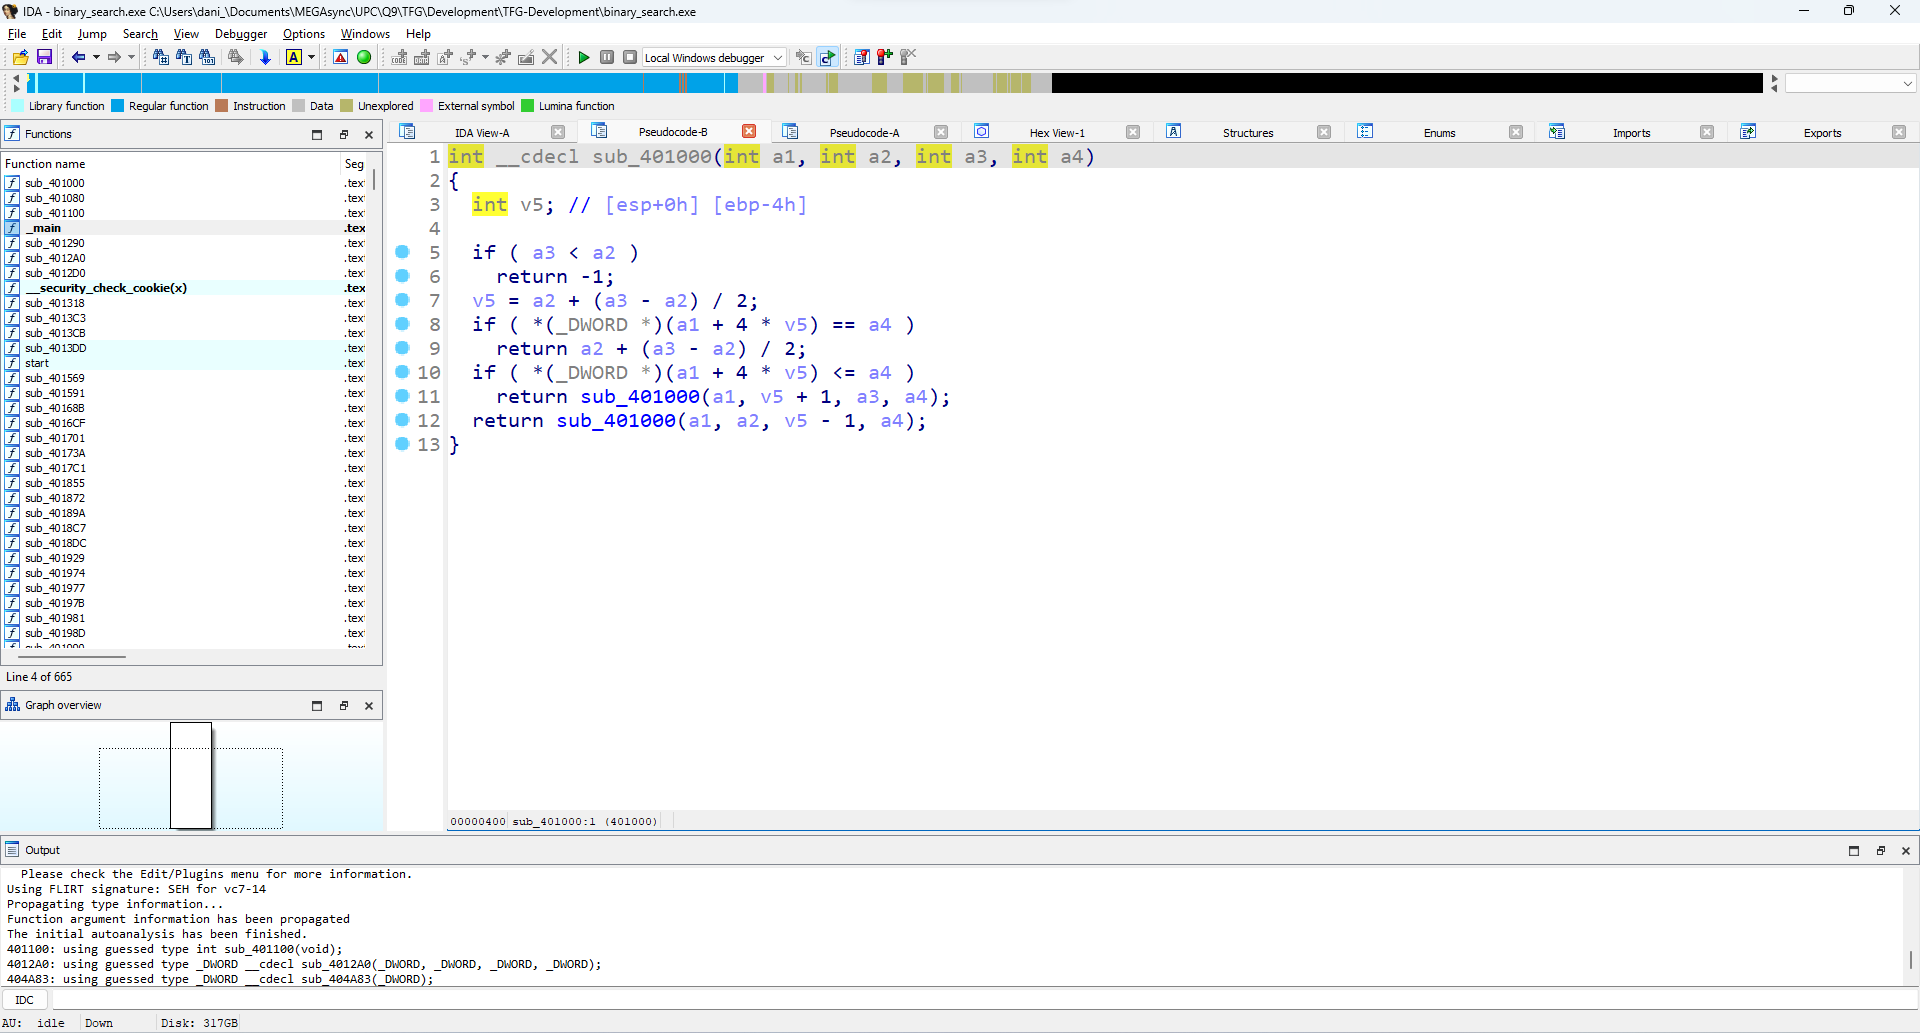
\includegraphics[width=15cm]{figuras/Capitulo_2/Cap_2_IDAPro_binaryseacrh1.png}
    \end{center}
    \caption[Captura de pantalla de IDA Free con el pseudocódigo generado para la funcion \textit{binaryseacrh1}]{Captura de pantalla de IDA Free con el pseudocódigo generado para la funcion \textit{binaryseacrh1} (Elaboración propia)}
    \label{fig:IDAPro_binaryseacrh1}
\end{figure}\

\begin{figure} [h!]
    \begin{center}
      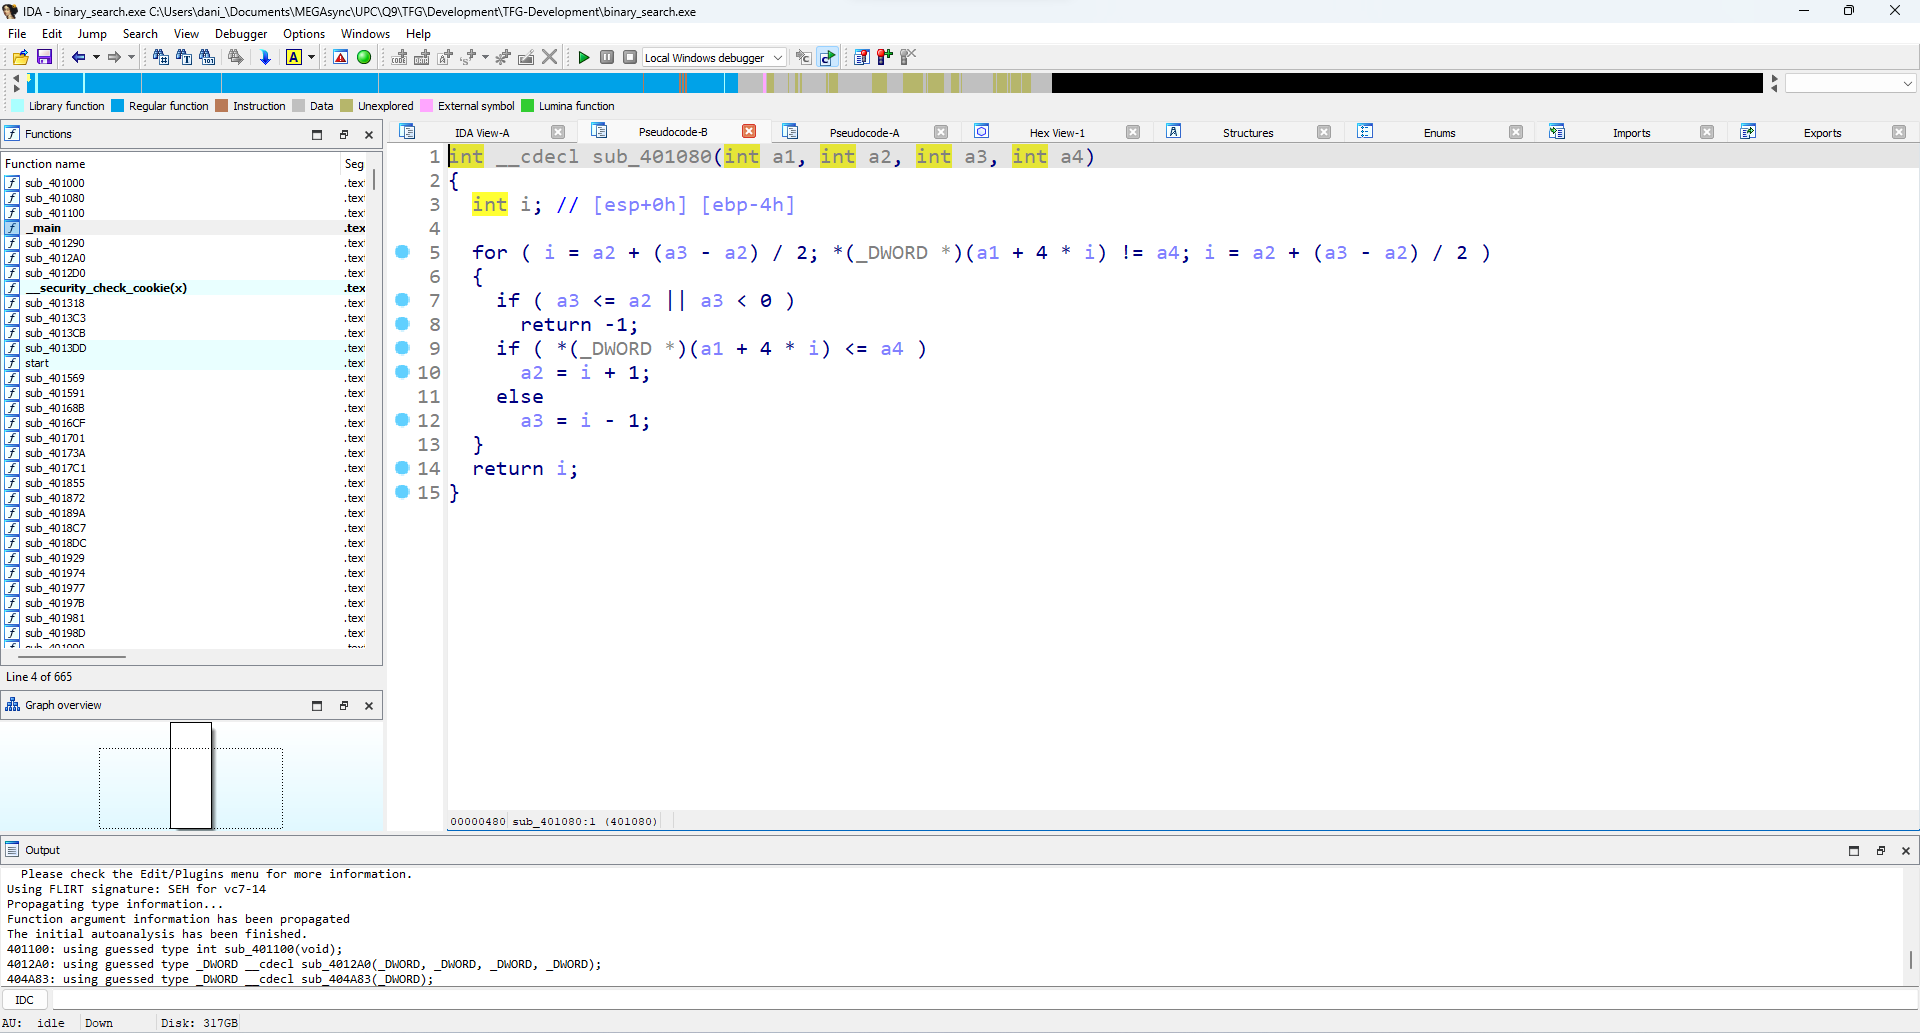
\includegraphics[width=15cm]{figuras/Capitulo_2/Cap_2_IDAPro_binaryseacrh2.png}
    \end{center}
    \caption[Captura de pantalla de IDA Free con el pseudocódigo generado para la funcion \textit{binaryseacrh2}]{Captura de pantalla de IDA Free con el pseudocódigo generado para la funcion \textit{binaryseacrh2} (Elaboración propia)}
    \label{fig:IDAPro_binaryseacrh2}
\end{figure}\

Observamos que el pseudocódigo que nos facilitan se asemeja al codigo original le queda ciertos aspectos en los cuales podria mejorar.

\section{Solucion tomada}
\label{sec:solucion}

% Corregido

La solución tomada pasa por investigar si el uso de inteligencia artificial, más concretamente el uso de modelos de lenguaje preentrenados, nos podría ayudar a la hora de hacer
ingeniería inversa sobre un programa en su forma de ejecutable u objeto.

Para poder hacerlo se decide utilizar modelos de lenguaje disponibles en Internet que la propia comunidad de desarrollo de software libre ha creado o modelos liberados por Microsoft.
La intención es aplicar \textit{fine-tuning} sobre estos modelos ya preentrenados, de tal manera que podemos aumentar la calidad de los resultados obtenidos para nuestra
tarea específica.

Así mismo, se tendrá que investigar sobre que método de \textit{fine-tuning} podemos utilizar, que se ajuste más a la características de nuestra tarea, teniendo en cuenta cosas como el
tipo de datos que se utilizan y el resultado que se quiere obtener.

% \chapter{Alcance}
\label{cap:alcance}

% Corregido

Al ser un proyecto que puede ser complejo y largo, definiremos el alcance y los objetivos que se deberán de cumplir para considerar que las hipótesis que nos
hemos planteado estén satisfechas.

\section{Objetivos}
\label{sec:objetivos}

% Corregido

Este proyecto tiene como objetivo principal investigar el uso de inteligencias artificiales para aplicar ingeniería inversa a programas.
En otras palabras, nos proponemos utilizar inteligencias artificiales tipo ChatGPT o similares para generar un código en C a partir única
y exclusivamente del ejecutable o de un archivo objeto.

Para poder alcanzar este objetivo se ha decidido dividirlo en subobjetivos, de tal manera que podamos ir dando pasos hasta el objetivo principal.
Los subobjetivos definidos son los siguientes:

\begin{itemize}
    \item Pruebas de uso con ChatGPT Plus, utilizando modelos como el GPT-3.5 y GPT-4
    \item Pruebas de uso con un modelo más pequeño denominados LoRA\footnote{LoRA (\textit{Low-Rank Adaptation}) es una técnica de \textit{fine-tuning} para modelos
        preentrenados en la cual propone utilizar una matriz de rangos baja de tal manera que reducimos los tiempos y memoria de GPU necesarios para el entrenamiento.}
        y haciendo \textit{fine-tuning} para nuestra tarea en específico.
\end{itemize}

El objetivo de realizar pruebas con ChatGPT es obtener una aproximación de los resultados que podamos obtener con nuestro modelo. ChatGPT nos
ofrece un entorno rápido y sencillo para poder hacer pruebas y analizar los resultados que podamos obtener.

Una vez realizadas las pruebas con ChatGPT, independientemente del resultado obtenido, se procederá a desplegar una inteligencia artificial más pequeña,
denominadas LoRa, en la cual se procederá a hacer diferentes métodos de \textit{fine-tuning}de tal manera que podemos aumentar la calidad de los resultados
obtenidos. La principal razón por la cual utilizamos modelos LoRa se debe a una cuestión técnica. Estos modelos están optimizados para obtener resultados
similares a un modelo normal como GPT-3.5 pero utilizando una cantidad menor de recursos hardware.

\section{Posibles riesgos y obstaculos}
\label{sec:riesgos}

% Corregido

Los riesgos que se asumen en este proyecto son altos debido a la incertidumbre que hay sobre este tema. Dado que los antecedentes son prácticamente nulos y dada una tecnología
que está en auge y aun en desarrollo, los posibles problemas o resultados no esperados que nos podamos encontrar durante la investigación y el desarrollo son altos.

Alguno de los posibles obstáculos que nos podemos encontrar son:

\begin{itemize}
    \item \textbf{Resultados no deseados:} podemos encontrarnos que a loa hora de querer generar código C a partir de un ejecutable el modelo no sea capaz de procesar estos datos
                                        y, por lo tanto, nos dé una salida que no es la esperada.
    \item \textbf{Insuficiencia de recursos:} los modelos que utilizaremos son modelos muy grandes que necesita mucha memoria de GPU para poderse ejecutar, aunque sabemos que
                                        existen modelos más pequeños y que necesitan menos recursos, podemos encontrarnos de que no sea suficiente esta reducción.
\end{itemize}
\chapter{Metodología y rigor}
\label{cap:metodologia}

\section{Metodología de trabajo}
\label{sec:metodologia:metodologia_trabajo}

En el desarrolo de este trabajo se utilizara una metodologia agil. En concreto, se utilizara 
la metodología SCRUM. as metodologías ágiles son aquellas que permiten dapatar la forma de
trabajo a las condiciones del proyecto, la cual cosa nos permite una mayor flexibilidad e 
inmediatez en la respuesta para amoldar el proyecto y su desarrollo a las circusntancias
especificas del entorno.

En concreto SCRUM es una metodología ágil que se basa en la división del trabajo en ciclos
llamados sprints. Estos sprints son periodos de tiempo en los que se desarrolla una parte
del proyecto. Al final de cada sprint se obtiene un producto funcional que puede ser entregado
al cliente. \cite{MetodoAgile}

Así mismo, este proyecto se dividira en diferentes etapas que se dividiran en sprints tal y
como se detalla en el capitulo \ref{cap:tareas}. Estas son las etapas que se han definido:

\begin{itemize}
    \item \textbf{Etapa de planificación:} En esta etapa se definiran los requisitos, 
    objetivos y tareas a realizar durante el proyecto.
    \item \textbf{Etapa de investigación:} En esta estapa se investigaran los posibles 
    resultados que se pueden obtener y se definiran las herramientas que se utilizaran.
    \item \textbf{Etapa de desarrollo:} En esta etapa se desarrollara todo el software 
    necesario para el proyecto.
    \item \textbf{Etapa de pruebas:} En esta etapa se realizaran las pruebas necesarias y los 
    ajustes necesarios para obtener los resultados deseados.
\end{itemize}

Durante todas las etapas se realizaran reuniónes de seguimiento con el Director del proyecto para
poder evaluar y correcgir las posibles desviaciones que se puedan producir.

\section{Seguimiento}
\label{sec:metodologia:seguimiento}



\chapter{Planificación}
\label{cap:planificacion}

% TODO:daniel: Añadir introducción

\section{Descripción de tareas}
\label{sec:descripcion_tareas}

% TODO:daniel: Canviar al nuevo formato

Para la realización de este proyecto se han creado diferentes tareas para la investigación, análisis y desarrollo de este mismo. La duración del proyecto está prevista
que tenga fecha de inicio el día 18 de septiembre de 2023 y con fecha de finalización el 22 de enero de 2024. El proyecto tendrá una dedicación de trabajo de unas 450 horas,
lo correspondiente a 18 créditos ECTS\footnote{Un crédito ECTS equivale a 25 horas de trabajo del estudiante.\cite{ECTS}}.

A continuación pasaré a detallar los paquetes de tareas y las tareas que componen cada paquete.

\subsection{Tareas de gestión del proyecto}
\label{subsec:tareas_gestion}

% Corregido

En las tareas de gestión del proyecto estarán todas las tareas que tengan que ver con gestión de proyectos, tales como definición del proyecto, presupuestos, reuniones de
sincronización, documentación relativa al proyecto, entre otras.

\subsubsection{Gestión del proyecto}
\label{subsubsec:tareas_gestion}

% Corregido

\begin{itemize}
    \item \textbf{Alcance}
        \begin{itemize}
            \item \textbf{Código:} GP01
            \item \textbf{Descripción:} Análisis y estudio del problema a estudiar, pudiendo definir el contexto y los objetivos del proyecto.
            \item \textbf{Duración:} 20h
            \item \textbf{Dependencias:} -
            \item \textbf{Recursos humanos:} Manager del proyecto
            \item \textbf{Recursos materiales:} Ordenador, Editor de texto
        \end{itemize}
    \item \textbf{Planificación}
        \begin{itemize}
            \item \textbf{Código:} GP02
            \item \textbf{Descripción:} Definición de plazos y tareas a realizar el proyecto, planificación temporal.
            \item \textbf{Duración:} 20h
            \item \textbf{Dependencias:} GP01
            \item \textbf{Recursos humanos:} Manager del proyecto
            \item \textbf{Recursos materiales:} Ordenador, Editor de texto
        \end{itemize}
    \item \textbf{Presupuesto}
        \begin{itemize}
            \item \textbf{Código:} GP03
            \item \textbf{Descripción:} Realización del coste del proyecto e informe de sostenibilidad.
            \item \textbf{Duración:} 20h
            \item \textbf{Dependencias:} GP02
            \item \textbf{Recursos humanos:} Manager del proyecto
            \item \textbf{Recursos materiales:} Ordenador, Editor de texto
        \end{itemize}
    \item \textbf{Evaluación del proyecto}
        \begin{itemize}
            \item \textbf{Código:} GP04
            \item \textbf{Descripción:} Revisar que la documentación aportada en las tareas GP01, GP02 y GP03 sea correcta y adecuada a los requisitos.
            \item \textbf{Duración:} 20h
            \item \textbf{Dependencias:} GP01, GP02, GP03
            \item \textbf{Recursos humanos:} Manager del proyecto
            \item \textbf{Recursos materiales:} Ordenador, Editor de texto
        \end{itemize}
    \item \textbf{Reuniones}
        \begin{itemize}
            \item \textbf{Código:} GP05
            \item \textbf{Descripción:} Reuniones de sincronización con el director del proyecto y con los expertos vinculados al proyecto.
            \item \textbf{Duración:} 20h
            \item \textbf{Dependencias:} - 
            \item \textbf{Recursos humanos:} Manager del proyecto, Director del proyecto
            \item \textbf{Recursos materiales:} Ordenador, Meet
        \end{itemize}
    \item \textbf{Documentación}
        \begin{itemize}
            \item \textbf{Código:} DC01
            \item \textbf{Descripción:} Creación, redactado y evaluación de la memoria de proyecto.
            \item \textbf{Duración:} 100h
            \item \textbf{Dependencias:} -
            \item \textbf{Recursos humanos:} Manager del proyecto
            \item \textbf{Recursos materiales:} Ordenador, Editor de texto
        \end{itemize}
\end{itemize}

\subsection{Tareas de análisis, investigación y pruebas}
\label{subsec:tareas_analisis}

% Corregido

Este paquete de tareas contempla todas aquellas tareas de investigación de documentación, tecnologías, análisis y realización de pruebas sobre nuevas tecnologías
que se puedan aplicar en nuestro caso de uso. En este caso, este paquete de tareas lo dividimos en tres: las tareas propias de investigación, las tareas propias de
análisis y las tareas relacionadas con \textit{deployment} de tecnologías.

\subsubsection{Investigación}
\label{subsubsec:tareas_investigacion}

% Corregido

\begin{itemize}
    \item \textbf{Investigación sobre el concepto LLMs}
        \begin{itemize}
            \item \textbf{Código:} I01
            \item \textbf{Descripción:} Investigación sobre los \textit{Large Language Models} y los conceptos asociados a este.
            \item \textbf{Duración:} 5h
            \item \textbf{Dependencias:} -
            \item \textbf{Recursos humanos:} Desarrolladores
            \item \textbf{Recursos materiales:} Ordenador
        \end{itemize}
    \item \textbf{Investigación LLMs Open Source}
        \begin{itemize}
            \item \textbf{Código:} I02
            \item \textbf{Descripción:} Investigación sobre los LLM disponibles creados por la comunidad, valorar cuál utilizar para el proyecto.
            \item \textbf{Duración:} 5h
            \item \textbf{Dependencias:} I01
            \item \textbf{Recursos humanos:} Desarrolladores
            \item \textbf{Recursos materiales:} Ordenador
        \end{itemize}
    \item \textbf{Investigación sobre métodos de \textit{fine-tuning}}
        \begin{itemize}
            \item \textbf{Código:} I03
            \item \textbf{Descripción:} Investigación sobre que metodo de \textit{fine-tuning} se ajusta más a las necesidades del proyecto.
            \item \textbf{Duración:} 5h
            \item \textbf{Dependencias:} I01
            \item \textbf{Recursos humanos:} Desarrolladores
            \item \textbf{Recursos materiales:} Ordenador, Git
        \end{itemize}
    \item \textbf{Recogida de datos para el entrenamiento}
        \begin{itemize}
            \item \textbf{Código:} I04
            \item \textbf{Descripción:} Investigación y análisis sobre repositorios de código, con código en C que sea apto para las pruebas en nuestro modelo. 
            \item \textbf{Duración:} 5h
            \item \textbf{Dependencias:} -
            \item \textbf{Recursos humanos:} Desarrolladores
            \item \textbf{Recursos materiales:} Ordenador, Git
        \end{itemize}
\end{itemize}

\subsubsection{Análisis y pruebas de uso utilizando ChatGPT Plus}
\label{subsubsec:tareas_ichatgpt}

% Corregido

\begin{itemize}
    \item \textbf{Análisis de ChatGPT}
        \begin{itemize}
            \item \textbf{Código:} AGPT01
            \item \textbf{Descripción:} Análisis sobre la plataforma de ChatGPT, como utilizar y obtener resultados óptimos.
            \item \textbf{Duración:} 4h
            \item \textbf{Dependencias:} -
            \item \textbf{Recursos humanos:} Desarrolladores
            \item \textbf{Recursos materiales:} Ordenador, ChatGPT Plus
        \end{itemize}
    \item \textbf{Pruebas de uso con GPT-3.5}
        \begin{itemize}
            \item \textbf{Código:} AGPT02
            \item \textbf{Descripción:} Pruebas con casos de código sencillo utilizando el modelo GPT-3.5 de ChatGPT Plus.
            \item \textbf{Duración:} 4h
            \item \textbf{Dependencias:} AGPT01
            \item \textbf{Recursos humanos:} Desarrolladores
            \item \textbf{Recursos materiales:} Ordenador, ChatGPT Plus
        \end{itemize}
    \item \textbf{Pruebas de uso con GPT-4}
        \begin{itemize}
            \item \textbf{Código:} AGPT03
            \item \textbf{Descripción:} Pruebas con casos de código sencillo utilizando el modelo GPT-4 de ChatGPT Plus.
            \item \textbf{Duración:} 4h
            \item \textbf{Dependencias:} AGPT01
            \item \textbf{Recursos humanos:} Desarrolladores
            \item \textbf{Recursos materiales:} Ordenador, ChatGPT Plus
        \end{itemize}
    \item \textbf{Análisis de los resultados}
        \begin{itemize}
            \item \textbf{Código:} AGPT04
            \item \textbf{Descripción:} Análisis de los resultados obtenidos en las pruebas de uso con GPT-3.5 y GPT-4, 
                valorando si obtendremos resultados buenos con nuestro modelo.
            \item \textbf{Duración:} 4h
            \item \textbf{Dependencias:} AGPT02, AGPT03
            \item \textbf{Recursos humanos:} Desarrolladores
            \item \textbf{Recursos materiales:} Ordenador
        \end{itemize}
\end{itemize}

\subsubsection{Deployment de un LLM en un sistema de GPUs}
\label{subsubsec:tareas_gpu}

% Corregido

\begin{itemize}
    \item \textbf{Análisis y pruebas de ejecución de un LLM}
        \begin{itemize}
            \item \textbf{Código:} D01
            \item \textbf{Descripción:} Ejecución de un LLM dentro de un \textit{cluster} de GPUs obteniendo resultados básicos, las pruebas que se hagan
                no tienen que estar relacionados con nuestros casos de uso.
            \item \textbf{Duración:} 28h
            \item \textbf{Dependencias:} I
            \item \textbf{Recursos humanos:} Desarrolladores
            \item \textbf{Recursos materiales:} Ordenador, Cluster AC
        \end{itemize}
    \item \textbf{Pruebas de ejecución de nuestro target}
        \begin{itemize}
            \item \textbf{Código:} D02
            \item \textbf{Descripción:} Ejecución de casos de uso sencillos en el \textit{cluster} de GPUs.
            \item \textbf{Duración:} 12h
            \item \textbf{Dependencias:} D01
            \item \textbf{Recursos humanos:} Desarrolladores
            \item \textbf{Recursos materiales:} Ordenador, Cluster AC
        \end{itemize}
    \item \textbf{\textit{Fine-tuning}}
        \begin{itemize}
            \item \textbf{Código:} D03
            \item \textbf{Descripción:} Ejecución del \textit{fine-tuning} sobre nuestro modelo de tal manera que obtengamos mejores resultados,
                en esta tarea se ha de utilizar el \textit{data sheet}.
            \item \textbf{Duración:} 20h
            \item \textbf{Dependencias:} D02, DH01
            \item \textbf{Recursos humanos:} Desarrolladores
            \item \textbf{Recursos materiales:} Ordenador, Cluster AC, Git
        \end{itemize}
    \item \textbf{Evaluación y correción 1}
        \begin{itemize}
            \item \textbf{Código:} D04
            \item \textbf{Descripción:} En esta tarea se valorarán los resultados obtenidos de la tarea D03 y se aplicaran las correcciones que sean
                necesarias.
            \item \textbf{Duración:} 20h
            \item \textbf{Dependencias:} D03
            \item \textbf{Recursos humanos:} Desarrolladores
            \item \textbf{Recursos materiales:} Ordenador, Cluster AC, Git
        \end{itemize}
    \item \textbf{Evaluación y correción 2}
        \begin{itemize}
            \item \textbf{Código:} D05
            \item \textbf{Descripción:} En esta tarea se valorarán los resultados obtenidos de la tarea D03 y se aplicaran las correcciones que sean
                necesarias.
            \item \textbf{Duración:} 40h
            \item \textbf{Dependencias:} D04
            \item \textbf{Recursos humanos:} Desarrolladores
            \item \textbf{Recursos materiales:} Ordenador, Cluster AC, Git
        \end{itemize}
\end{itemize}

\subsection{Tareas de desarrollo}
\label{subsec:tareas_desarrollo}

% Corregido 

En este grupo de tareas situaremos todas aquellas relacionadas con el desarrollo, ya sea el desarrollo de herramientas que ayudan a la hora del desarrollo en
sí mismo, o tareas más de creación de aplicaciones o similares.

\subsubsection{Desarrollo de herramientas}
\label{subsubsec:tareas_herramientas}

% Corregido 

\begin{itemize}
    \item \textbf{Desarrollo de scripts para la creación del Data Sheet}
        \begin{itemize}
            \item \textbf{Código:} DH01
            \item \textbf{Descripción:} Desarrollo de scripts para compilar, parsear y obtener los ensamblados. Así mismo, se creara la base de datos
                necesaria para el \textit{fine-tuning}.
            \item \textbf{Duración:} 28h
            \item \textbf{Dependencias:} -
            \item \textbf{Recursos humanos:} Desarrolladores
            \item \textbf{Recursos materiales:} Ordenador, Git
        \end{itemize}
    \item \textbf{Desarrollo de scripts de ejecución}
        \begin{itemize}
            \item \textbf{Código:} DH02
            \item \textbf{Descripción:} Desarrollo de scripts para la ejecución del LLM en el \textit{cluster} de GPUs.
            \item \textbf{Duración:} 20h
            \item \textbf{Dependencias:} -
            \item \textbf{Recursos humanos:} Desarrolladores
            \item \textbf{Recursos materiales:} Ordenador, Cluster AC, Git
        \end{itemize}
\end{itemize}

\section{Recursos}
\label{subsec:recursos}

% Corregido

En esta sección se detallarán los recursos que se utilizarán para la realización de este proyecto, distinguiremos entre dos tipos
de recursos: recursos humanos que son aquellos actores implicados en el proyecto de forma directa o indirecta, y recursos materiales
que son aquellos recursos que se utilizarán para la realización del proyecto.

\subsection{Recursos humanos}
\label{subsec:recursos_humanos}

% Corregido

La lista de recursos humanos que se utilizarán para la realización de este proyecto son los siguientes:

\begin{itemize}
    \item \textbf{Director del proyecto:} Este recurso es el encargado de dirigir el proyecto, así mismo, es el encargado de la supervisión del proyecto.
    \item \textbf{Manager del proyecto:} Este recurso es el encargado de la gestión del proyecto, así mismo, es el encargado de la gestión de los recursos
        humanos y materiales.
    \item \textbf{Desarrolladores:} Este recurso es el encargado de la realización de las tareas de desarrollo, así mismo, es el encargado de la realización
        de las tareas de investigación y análisis.
\end{itemize}

\subsection{Recursos materiales}
\label{subsec:recursos_materiales}

% Corregido

La lista de recursos materiales que se utilizarán para la realización de este proyecto son los siguientes:

\begin{itemize}
    \item \textbf{Ordenador:} Este recurso es el encargado de la realización de las tareas de investigación, análisis y desarrollo.
    \item \textbf{Editor de texto:} Este recurso es el encargado de la realización de las tareas de documentación.
    \item \textbf{GitHub:} Este recurso es el encargado de la realización de las tareas de documentación.
    \item \textbf{Meet:} Este recurso es el encargado de la realización de las tareas de reuniones.
    \item \textbf{Cluster AC:} Este recurso es el encargado de la realización de las tareas de ejecución de los LLMs.
    \item \textbf{ChatGPT Plus:} Este recurso es el encargado de la realización de las tareas de análisis y pruebas de uso utilizando ChatGPT Plus.
\end{itemize}

\section{Estimación del proyecto}
\label{sec:estimacion}

% Corregido

Como hemos mencionado en el capítulo \ref{cap:tareas}, el proyecto tiene una duración de 4 meses, en la cual se estiman unas 475 horas de trabajo, en las cuales se
comprenden tareas de gestión de proyectos, documentación, investigación, análisis, realización de pruebas y desarrollo. Así mismo, siendo conscientes de que un proyecto
tiene riesgos e imprevistos, y tal como exponemos en el capítulo \ref{sec:riesgos}, disponemos de un margen de 144 horas que podemos utilizar, pero que dentro de este
capítulo no se ven reflejadas.

El proyecto se ha dividido en 7 periodos, seis de ellos son \textit{sprints} de 3 semanas de duración, empezando el primero el día 18 de septiembre de 2023 y acabando el último
el día 22 de enero de 2024, y un periodo de una semana que será el periodo de defensa del proyecto.

Cada \textit{sprint} se compone de 3 semanas, estas semanas van de lunes a viernes y donde cada día disponemos de 4 horas de trabajo efectivo, convirtiéndose en 20 horas semanas
y en 60 horas por \textit{sprint}. Así mismo, en cada sprint disponemos de 24 horas de margen en caso de surgir un imprevisto o contratiempo.

La fecha de finalización del proyecto será una semana antes de la defensa del proyecto, siendo está dentro de la última semana del \textit{sprint} número 6.

Por lo tanto, en la siguiente tabla \ref{tab:proyecto_estimacion} disponemos un resumen de las fechas de cada periodo de este proyecto.

\begin{table}[H]
    \centering
    \begin{tabular}{|l|l|l|}
    \hline
    \rowcolor[HTML]{8EA9D8} 
    Sprints      & Fecha de inicio & Fecha de finalización \\ \hline
    Sprint 01    & 18/09/2023      & 09/10/2023            \\ \hline
    Sprint 02    & 09/10/2023      & 30/10/2023            \\ \hline
    Sprint 03    & 30/10/2023      & 20/11/2023            \\ \hline
    Sprint 04    & 20/11/2023      & 11/12/2023            \\ \hline
    Sprint 05    & 11/12/2023      & 01/01/2024            \\ \hline
    Sprint 06    & 01/01/2024      & 22/01/2024            \\ \hline
    Presentación & 22/01/2024      & 26/01/2024            \\ \hline
    \end{tabular}
    \caption[División del proyecto por sprints]{División del proyecto por sprints (Elaboración propia)}
    \label{tab:proyecto_estimacion}
\end{table}

\subsection{Estimación de tareas}
\label{sec:estimacion_tareas}

% Corregido

La siguiente tabla \ref{tab:tareas} podréis ver un resumen de las tareas especificadas para este proyecto con la correspondiente estimación. En total,
la duración del proyecto será de 475 horas, en las cuales no se contempla ningún imprevisto, en casa de imprevisto se procederá con el protocolo definido
en el capítulo \ref{cap:riesgos}.

En modo de leyenda, en esta tabla \ref{tab:recursos} podréis ver cuáles son los recursos disponibles.

\begin{table}[H]
    \centering
    \begin{tabular}{|l|l|}
    \hline
    \rowcolor[HTML]{8EA9D8} 
    Código & Recurso                        \\ \hline
    PC     & Ordenador                      \\ \hline
    G      & GitHub                         \\ \hline
    ET     & Editor de texto                \\ \hline
    MT     & Meet                           \\ \hline
    CAC    & Cluster del departamento de AC \\ \hline
    GPT    & ChatGPT Plus                   \\ \hline
    DR     & Director del proyecto          \\ \hline
    M      & Manager del proyecto           \\ \hline
    D      & Desarrolladores                \\ \hline
    \end{tabular}
    \caption[Recursos del proyecto con su respectivo código]{Recursos del proyecto con su respectivo código (Elaboración propia)}
    \label{tab:recursos}
\end{table}

\begin{table}[H]
    \centering
    \resizebox{\textwidth}{!}{%
    \begin{tabular}{|llcll|}
    \hline
    \rowcolor[HTML]{8EA9D8} 
    \multicolumn{1}{|c|}{\cellcolor[HTML]{8EA9D8}\textbf{Código}} & \multicolumn{1}{c|}{\cellcolor[HTML]{8EA9D8}\textbf{Nombre tarea}}         & \multicolumn{1}{c|}{\cellcolor[HTML]{8EA9D8}\textbf{Horas de trabajo}} & \multicolumn{1}{c|}{\cellcolor[HTML]{8EA9D8}\textbf{Dependencias}} & \multicolumn{1}{c|}{\cellcolor[HTML]{8EA9D8}\textbf{Recursos}} \\ \hline
    \multicolumn{1}{|l|}{\textbf{GP}}                             & \multicolumn{4}{l|}{\textbf{Gestión del proyecto}}                                                                                                                                                                                                                                        \\ \hline
    \multicolumn{1}{|l|}{GP01}                                    & \multicolumn{1}{l|}{Alcance}                                               & \multicolumn{1}{c|}{20}                                                & \multicolumn{1}{l|}{-}                                             & PC, ET, M                                                      \\ \hline
    \multicolumn{1}{|l|}{GP02}                                    & \multicolumn{1}{l|}{Planificación}                                         & \multicolumn{1}{c|}{20}                                                & \multicolumn{1}{l|}{GP01}                                          & PC, ET, M                                                      \\ \hline
    \multicolumn{1}{|l|}{GP03}                                    & \multicolumn{1}{l|}{Presupuesto}                                           & \multicolumn{1}{c|}{20}                                                & \multicolumn{1}{l|}{GP02}                                          & PC, ET, M                                                      \\ \hline
    \multicolumn{1}{|l|}{GP04}                                    & \multicolumn{1}{l|}{Evaluación del proyecto}                               & \multicolumn{1}{c|}{20}                                                & \multicolumn{1}{l|}{GP01, GP02, GP03}                              & PC, ET, M                                                      \\ \hline
    \multicolumn{1}{|l|}{GP05}                                    & \multicolumn{1}{l|}{Reuniones}                                             & \multicolumn{1}{c|}{20}                                                & \multicolumn{1}{l|}{-}                                             & PC, MT, DR, M                                                  \\ \hline
    \multicolumn{1}{|l|}{DC01}                                    & \multicolumn{1}{l|}{Documentación}                                         & \multicolumn{1}{c|}{176}                                               & \multicolumn{1}{l|}{-}                                             & PC, ET, G, M                                                   \\ \hline
    \rowcolor[HTML]{8EA9D8} 
    \multicolumn{2}{|l|}{\cellcolor[HTML]{8EA9D8}Total horas paquete}                                                                          & 276                                                                    &                                                                    &                                                                \\ \hline
    \multicolumn{1}{|l|}{\textbf{I}}                              & \multicolumn{4}{l|}{\textbf{Investigación y analisis}}                                                                                                                                                                                                                                    \\ \hline
    \multicolumn{1}{|l|}{I01}                                     & \multicolumn{1}{l|}{Investigación sobre el concepto LLMs}                  & \multicolumn{1}{c|}{5}                                                 & \multicolumn{1}{l|}{-}                                             & PC, D                                                          \\ \hline
    \multicolumn{1}{|l|}{I02}                                     & \multicolumn{1}{l|}{Investigación LLMs Open Source}                        & \multicolumn{1}{c|}{5}                                                 & \multicolumn{1}{l|}{I01}                                           & PC, D                                                          \\ \hline
    \multicolumn{1}{|l|}{I03}                                     & \multicolumn{1}{l|}{Investigación sobre métodos de fine-tuning}            & \multicolumn{1}{c|}{5}                                                 & \multicolumn{1}{l|}{I01}                                           & PC, D                                                          \\ \hline
    \multicolumn{1}{|l|}{I04}                                     & \multicolumn{1}{l|}{Recogida de datos para el entrenamiento}               & \multicolumn{1}{c|}{5}                                                 & \multicolumn{1}{l|}{-}                                             & PC, G, D                                                       \\ \hline
    \rowcolor[HTML]{8EA9D8} 
    \multicolumn{2}{|l|}{\cellcolor[HTML]{8EA9D8}Total horas paquete}                                                                          & 20                                                                     &                                                                    &                                                                \\ \hline
    \multicolumn{1}{|l|}{\textbf{AGPT}}                           & \multicolumn{4}{l|}{\textbf{Análisis y pruebas de la solución utilizando ChatGPT Plus}}                                                                                                                                                                                                   \\ \hline
    \multicolumn{1}{|l|}{AGPT01}                                  & \multicolumn{1}{l|}{Análisis de ChatGPT}                                   & \multicolumn{1}{c|}{4}                                                 & \multicolumn{1}{l|}{-}                                             & PC, GPT, D                                                     \\ \hline
    \multicolumn{1}{|l|}{AGPT02}                                  & \multicolumn{1}{l|}{Pruebas de uso con GPT-3.5}                            & \multicolumn{1}{c|}{4}                                                 & \multicolumn{1}{l|}{AGPT01}                                        & PC, GPT, D                                                     \\ \hline
    \multicolumn{1}{|l|}{AGPT03}                                  & \multicolumn{1}{l|}{Pruebas de uso con GPT-4}                              & \multicolumn{1}{c|}{4}                                                 & \multicolumn{1}{l|}{AGPT01}                                        & PC, GPT, D                                                     \\ \hline
    \multicolumn{1}{|l|}{AGPT04}                                  & \multicolumn{1}{l|}{Analisis de los resultados}                            & \multicolumn{1}{c|}{4}                                                 & \multicolumn{1}{l|}{AGPT02, AGPT03}                                & PC, D                                                          \\ \hline
    \rowcolor[HTML]{8EA9D8} 
    \multicolumn{2}{|l|}{\cellcolor[HTML]{8EA9D8}Total horas paquete}                                                                          & 16                                                                     &                                                                    &                                                                \\ \hline
    \multicolumn{1}{|l|}{\textbf{D}}                              & \multicolumn{4}{l|}{\textbf{Deployment de un LLM en un sistema de GPUs}}                                                                                                                                                                                                                  \\ \hline
    \multicolumn{1}{|l|}{D01}                                     & \multicolumn{1}{l|}{Análisis y pruebas de ejecución de un LLM}             & \multicolumn{1}{c|}{28}                                                & \multicolumn{1}{l|}{I}                                             & PC, CAC, D                                                     \\ \hline
    \multicolumn{1}{|l|}{D02}                                     & \multicolumn{1}{l|}{Pruebas de ejecución de nuestro target}                & \multicolumn{1}{c|}{12}                                                & \multicolumn{1}{l|}{D01}                                           & PC, CAC, D                                                     \\ \hline
    \multicolumn{1}{|l|}{D03}                                     & \multicolumn{1}{l|}{Fine-tuning}                                           & \multicolumn{1}{c|}{20}                                                & \multicolumn{1}{l|}{D02, DH01}                                     & PC, CAC, G, D                                                  \\ \hline
    \multicolumn{1}{|l|}{D04}                                     & \multicolumn{1}{l|}{Evaluación y correción 1}                              & \multicolumn{1}{c|}{20}                                                & \multicolumn{1}{l|}{D03}                                           & PC, CAC, G, D                                                  \\ \hline
    \multicolumn{1}{|l|}{D05}                                     & \multicolumn{1}{l|}{Evaluación y correción 2}                              & \multicolumn{1}{c|}{40}                                                & \multicolumn{1}{l|}{D04}                                           & PC, CAC, G, D                                                  \\ \hline
    \rowcolor[HTML]{8EA9D8} 
    \multicolumn{2}{|l|}{\cellcolor[HTML]{8EA9D8}Total horas paquete}                                                                          & 120                                                                    &                                                                    &                                                                \\ \hline
    \multicolumn{1}{|l|}{\textbf{DH}}                             & \multicolumn{4}{l|}{\textbf{Desarrollo de herramientas}}                                                                                                                                                                                                                                  \\ \hline
    \multicolumn{1}{|l|}{DH01}                                    & \multicolumn{1}{l|}{Desarrollo de scripts para la creación del Data Sheet} & \multicolumn{1}{c|}{28}                                                & \multicolumn{1}{l|}{-}                                             & PC, G, D                                                       \\ \hline
    \multicolumn{1}{|l|}{DH02}                                    & \multicolumn{1}{l|}{Desarrollo de scripts de ejecución}                    & \multicolumn{1}{c|}{18}                                                & \multicolumn{1}{l|}{-}                                             & PC, CAC, G, D                                                  \\ \hline
    \rowcolor[HTML]{8EA9D8} 
    \multicolumn{2}{|l|}{\cellcolor[HTML]{8EA9D8}Total horas paquete}                                                                          & 46                                                                     &                                                                    &                                                                \\ \hline
    \rowcolor[HTML]{305496} 
    \multicolumn{2}{|l|}{\cellcolor[HTML]{305496}Total horas}                                                                                  & \multicolumn{1}{c|}{\cellcolor[HTML]{305496}478}                       &                                                                    &                                                                \\ \hline
    \end{tabular}%
    }
    \caption[Resumen de las tareas del proyecto]{Resumen de las tareas del proyecto (Elaboración propia)}
    \label{tab:tareas}
\end{table}

\newpage
\paperwidth=\pdfpageheight
\paperheight=\pdfpagewidth
\pdfpageheight=\paperheight
\pdfpagewidth=\paperwidth
\headwidth=\textheight

\begingroup
    \vsize=\textwidth
    \hsize=\textheight
    \subsubsection{Diagrama de Gantt}
    \label{sec:gantt}
    \begin{table}[h]
        \centering
        \begin{tabular}{|llcllllllllllllllll|}
        \hline
        \multicolumn{19}{|c|}{\cellcolor[HTML]{8EA9D8}\textbf{Sprint 01}}                                                                                                                                                                                                                                                                                                                                                                                                                                                                                                                                                                                                                                                                                                                                                                                                                            \\ \hline
        \multicolumn{1}{|c|}{\cellcolor[HTML]{FFFFFF}}                                                             & \multicolumn{1}{c|}{\cellcolor[HTML]{FFFFFF}}                                  & \multicolumn{1}{c|}{\cellcolor[HTML]{FFFFFF}}                                    & \multicolumn{1}{c|}{\cellcolor[HTML]{FFFFFF}}                                        & \multicolumn{5}{c|}{\cellcolor[HTML]{FFFFFF}\textbf{Sep 18}}                                                                                                            & \multicolumn{5}{c|}{\cellcolor[HTML]{FFFFFF}\textbf{Sep 25}}                                                                                                            & \multicolumn{5}{c|}{\cellcolor[HTML]{FFFFFF}\textbf{Oct 02}}                                                                                                     \\ \cline{5-19} 
        \multicolumn{1}{|c|}{\multirow{-2}{*}{\cellcolor[HTML]{FFFFFF}\textbf{Nombre tarea}}}                      & \multicolumn{1}{c|}{\multirow{-2}{*}{\cellcolor[HTML]{FFFFFF}\textbf{Código}}} & \multicolumn{1}{c|}{\multirow{-2}{*}{\cellcolor[HTML]{FFFFFF}\textbf{Duración}}} & \multicolumn{1}{c|}{\multirow{-2}{*}{\cellcolor[HTML]{FFFFFF}\textbf{Dependencias}}} & \multicolumn{1}{l|}{\textit{L}} & \multicolumn{1}{l|}{\textit{M}} & \multicolumn{1}{l|}{\textit{X}} & \multicolumn{1}{l|}{\textit{J}} & \multicolumn{1}{l|}{\textit{V}} & \multicolumn{1}{l|}{\textit{L}} & \multicolumn{1}{l|}{\textit{M}} & \multicolumn{1}{l|}{\textit{X}} & \multicolumn{1}{l|}{\textit{J}} & \multicolumn{1}{l|}{\textit{V}} & \multicolumn{1}{l|}{\textit{L}} & \multicolumn{1}{l|}{\textit{M}} & \multicolumn{1}{l|}{\textit{X}} & \multicolumn{1}{l|}{\textit{J}} & \textit{V}               \\ \hline
        \multicolumn{4}{|l|}{\textbf{Gestión del proyecto}}                                                                                                                                                                                                                                                                                                                   & \multicolumn{15}{l|}{}                                                                                                                                                                                                                                                                                                                                                                                                                                                                                               \\ \hline
        \multicolumn{1}{|l|}{Alcance}                                                                              & \multicolumn{1}{l|}{GP01}                                                      & \multicolumn{1}{c|}{1}                                                           & \multicolumn{1}{l|}{-}                                                               & \cellcolor[HTML]{C6E0B4}        & \cellcolor[HTML]{C6E0B4}        & \cellcolor[HTML]{C6E0B4}        & \cellcolor[HTML]{C6E0B4}        & \cellcolor[HTML]{C6E0B4}        &                                 &                                 &                                 &                                 &                                 &                                 &                                 &                                 &                                 &                          \\ \cline{1-4}
        \multicolumn{1}{|l|}{Planificación}                                                                        & \multicolumn{1}{l|}{GP02}                                                      & \multicolumn{1}{c|}{1}                                                           & \multicolumn{1}{l|}{GP01}                                                            &                                 &                                 &                                 &                                 &                                 & \cellcolor[HTML]{C6E0B4}        & \cellcolor[HTML]{C6E0B4}        & \cellcolor[HTML]{C6E0B4}        & \cellcolor[HTML]{C6E0B4}        & \cellcolor[HTML]{C6E0B4}        &                                 &                                 &                                 &                                 &                          \\ \cline{1-4}
        \multicolumn{1}{|l|}{Presupuesto}                                                                          & \multicolumn{1}{l|}{GP03}                                                      & \multicolumn{1}{c|}{1}                                                           & \multicolumn{1}{l|}{GP02}                                                            &                                 &                                 &                                 &                                 &                                 &                                 &                                 &                                 &                                 &                                 & \cellcolor[HTML]{C6E0B4}        & \cellcolor[HTML]{C6E0B4}        & \cellcolor[HTML]{C6E0B4}        & \cellcolor[HTML]{C6E0B4}        & \cellcolor[HTML]{C6E0B4} \\ \cline{1-4}
        \multicolumn{1}{|l|}{Reuniones}                                                                            & \multicolumn{1}{l|}{GP05}                                                      & \multicolumn{1}{c|}{0.4}                                                         & \multicolumn{1}{l|}{-}                                                               &                                 &                                 &                                 & \cellcolor[HTML]{EF8787}        &                                 &                                 &                                 &                                 &                                 &                                 &                                 &                                 &                                 & \cellcolor[HTML]{EF8787}        &                          \\ \cline{1-4}
        \multicolumn{1}{|l|}{Documentación}                                                                        & \multicolumn{1}{l|}{DC01}                                                      & \multicolumn{1}{c|}{3}                                                           & \multicolumn{1}{l|}{-}                                                               & \cellcolor[HTML]{C9C9C9}        & \cellcolor[HTML]{C9C9C9}        & \cellcolor[HTML]{C9C9C9}        & \cellcolor[HTML]{C9C9C9}        & \cellcolor[HTML]{C9C9C9}        & \cellcolor[HTML]{C9C9C9}        & \cellcolor[HTML]{C9C9C9}        & \cellcolor[HTML]{C9C9C9}        & \cellcolor[HTML]{C9C9C9}        & \cellcolor[HTML]{C9C9C9}        & \cellcolor[HTML]{C9C9C9}        & \cellcolor[HTML]{C9C9C9}        & \cellcolor[HTML]{C9C9C9}        & \cellcolor[HTML]{C9C9C9}        & \cellcolor[HTML]{C9C9C9} \\ \hline
        \multicolumn{19}{|c|}{\cellcolor[HTML]{8EA9D8}\textbf{Sprint 02}}                                                                                                                                                                                                                                                                                                                                                                                                                                                                                                                                                                                                                                                                                                                                                                                                                            \\ \hline
        \multicolumn{1}{|c|}{\cellcolor[HTML]{FFFFFF}}                                                             & \multicolumn{1}{c|}{\cellcolor[HTML]{FFFFFF}}                                  & \multicolumn{1}{c|}{\cellcolor[HTML]{FFFFFF}}                                    & \multicolumn{1}{c|}{\cellcolor[HTML]{FFFFFF}}                                        & \multicolumn{5}{c|}{\textbf{Oct 09}}                                                                                                                                    & \multicolumn{5}{c|}{\textbf{Oct 16}}                                                                                                                                    & \multicolumn{5}{c|}{\textbf{Oct 23}}                                                                                                                             \\ \cline{5-19} 
        \multicolumn{1}{|c|}{\multirow{-2}{*}{\cellcolor[HTML]{FFFFFF}\textbf{Nombre tarea}}}                      & \multicolumn{1}{c|}{\multirow{-2}{*}{\cellcolor[HTML]{FFFFFF}\textbf{Código}}} & \multicolumn{1}{c|}{\multirow{-2}{*}{\cellcolor[HTML]{FFFFFF}\textbf{Duración}}} & \multicolumn{1}{c|}{\multirow{-2}{*}{\cellcolor[HTML]{FFFFFF}\textbf{Dependencias}}} & \multicolumn{1}{l|}{\textit{L}} & \multicolumn{1}{l|}{\textit{M}} & \multicolumn{1}{l|}{\textit{X}} & \multicolumn{1}{l|}{\textit{J}} & \multicolumn{1}{l|}{\textit{V}} & \multicolumn{1}{l|}{\textit{L}} & \multicolumn{1}{l|}{\textit{M}} & \multicolumn{1}{l|}{\textit{X}} & \multicolumn{1}{l|}{\textit{J}} & \multicolumn{1}{l|}{\textit{V}} & \multicolumn{1}{l|}{\textit{L}} & \multicolumn{1}{l|}{\textit{M}} & \multicolumn{1}{l|}{\textit{X}} & \multicolumn{1}{l|}{\textit{J}} & \textit{V}               \\ \hline
        \multicolumn{4}{|l|}{\textbf{Gestión del proyecto}}                                                                                                                                                                                                                                                                                                                   & \multicolumn{15}{l|}{}                                                                                                                                                                                                                                                                                                                                                                                                                                                                                               \\ \hline
        \multicolumn{1}{|l|}{\begin{tabular}[c]{@{}l@{}}Evaluación del\\ proyecto\end{tabular}}                    & \multicolumn{1}{l|}{GP04}                                                      & \multicolumn{1}{c|}{1}                                                           & \multicolumn{1}{l|}{\begin{tabular}[c]{@{}l@{}}GP01\\ GP02\\ GP03\end{tabular}}      & \cellcolor[HTML]{C6E0B4}        & \cellcolor[HTML]{C6E0B4}        & \cellcolor[HTML]{C6E0B4}        & \cellcolor[HTML]{C6E0B4}        & \cellcolor[HTML]{C6E0B4}        &                                 &                                 &                                 &                                 &                                 &                                 &                                 &                                 &                                 &                          \\ \cline{1-4}
        \multicolumn{1}{|l|}{Reuniones}                                                                            & \multicolumn{1}{l|}{GP05}                                                      & \multicolumn{1}{c|}{0.2}                                                         & \multicolumn{1}{l|}{-}                                                               &                                 &                                 &                                 &                                 &                                 &                                 &                                 &                                 & \cellcolor[HTML]{EF8787}        &                                 &                                 &                                 &                                 &                                 &                          \\ \cline{1-4}
        \multicolumn{1}{|l|}{Documentación}                                                                        & \multicolumn{1}{l|}{DC01}                                                      & \multicolumn{1}{c|}{2}                                                           & \multicolumn{1}{l|}{-}                                                               & \cellcolor[HTML]{C9C9C9}        & \cellcolor[HTML]{C9C9C9}        & \cellcolor[HTML]{C9C9C9}        & \cellcolor[HTML]{C9C9C9}        & \cellcolor[HTML]{C9C9C9}        &                                 &                                 &                                 & \cellcolor[HTML]{FFFFFF}        & \cellcolor[HTML]{FFFFFF}        & \cellcolor[HTML]{C9C9C9}        & \cellcolor[HTML]{C9C9C9}        & \cellcolor[HTML]{C9C9C9}        & \cellcolor[HTML]{C9C9C9}        & \cellcolor[HTML]{C9C9C9} \\ \hline
        \multicolumn{4}{|l|}{\textbf{Investigación y analisis}}                                                                                                                                                                                                                                                                                                               & \multicolumn{15}{l|}{}                                                                                                                                                                                                                                                                                                                                                                                                                                                                                               \\ \hline
        \multicolumn{1}{|l|}{\begin{tabular}[c]{@{}l@{}}Investigación sobre\\ el concepto LLM\end{tabular}}        & \multicolumn{1}{l|}{I01}                                                       & \multicolumn{1}{c|}{0.8}                                                         & \multicolumn{1}{l|}{-}                                                               &                                 &                                 &                                 &                                 &                                 & \cellcolor[HTML]{A9D08E}        & \cellcolor[HTML]{A9D08E}        &                                 &                                 &                                 &                                 &                                 &                                 &                                 &                          \\ \cline{1-4}
        \multicolumn{1}{|l|}{\begin{tabular}[c]{@{}l@{}}Investigación LLMs\\ Open Source\end{tabular}}             & \multicolumn{1}{l|}{I02}                                                       & \multicolumn{1}{c|}{0.8}                                                         & \multicolumn{1}{l|}{I01}                                                             &                                 &                                 &                                 &                                 &                                 &                                 & \cellcolor[HTML]{A9D08E}        & \cellcolor[HTML]{A9D08E}        &                                 &                                 &                                 &                                 &                                 &                                 &                          \\ \cline{1-4}
        \multicolumn{1}{|l|}{\begin{tabular}[c]{@{}l@{}}Investigación sobre\\ métodos de fine-tuning\end{tabular}} & \multicolumn{1}{l|}{I03}                                                       & \multicolumn{1}{c|}{0.8}                                                         & \multicolumn{1}{l|}{I01}                                                             &                                 &                                 &                                 &                                 &                                 &                                 &                                 & \cellcolor[HTML]{A9D08E}        & \cellcolor[HTML]{A9D08E}        &                                 &                                 &                                 &                                 &                                 &                          \\ \cline{1-4}
        \multicolumn{1}{|l|}{\begin{tabular}[c]{@{}l@{}}Recogida de datos\\ para el entrenamiento\end{tabular}}    & \multicolumn{1}{l|}{I04}                                                       & \multicolumn{1}{c|}{0.8}                                                         & \multicolumn{1}{l|}{-}                                                               &                                 &                                 &                                 &                                 &                                 &                                 &                                 &                                 & \cellcolor[HTML]{A9D08E}        & \cellcolor[HTML]{A9D08E}        &                                 &                                 &                                 &                                 &                          \\ \hline
        \end{tabular}
        \caption[Diagrama de Gantt Sprint 01 - Sprint 02]{Diagrama de Gantt Sprint 01 - Sprint 02 (Elaboración propia)}
        \label{tab:Diagrama_gantt_01-02}
    \end{table}

    \begin{table}[H]
        \centering
        \begin{tabular}{|llcllllllllllllllll|}
        \hline
        \multicolumn{19}{|c|}{\cellcolor[HTML]{8EA9D8}\textbf{Sprint 03}}                                                                                                                                                                                                                                                                                                                                                                                                                                                                                                                                                                                                                                                                                                                                                                                 \\ \hline
        \multicolumn{1}{|c|}{}                                                                                                  & \multicolumn{1}{c|}{}                                  & \multicolumn{1}{c|}{}                                    & \multicolumn{1}{c|}{}                                                        & \multicolumn{5}{c|}{\textbf{Oct 30}}                                                                                                                                    & \multicolumn{5}{c|}{\textbf{Nov 06}}                                                                                                                                    & \multicolumn{5}{c|}{\textbf{Nov 13}}                                                                                                                             \\ \cline{5-19} 
        \multicolumn{1}{|c|}{\multirow{-2}{*}{\textbf{Nombre tarea}}}                                                           & \multicolumn{1}{c|}{\multirow{-2}{*}{\textbf{Código}}} & \multicolumn{1}{c|}{\multirow{-2}{*}{\textbf{Duración}}} & \multicolumn{1}{c|}{\multirow{-2}{*}{\textbf{Dependencias}}}                 & \multicolumn{1}{l|}{\textit{L}} & \multicolumn{1}{l|}{\textit{M}} & \multicolumn{1}{l|}{\textit{X}} & \multicolumn{1}{l|}{\textit{J}} & \multicolumn{1}{l|}{\textit{V}} & \multicolumn{1}{l|}{\textit{L}} & \multicolumn{1}{l|}{\textit{M}} & \multicolumn{1}{l|}{\textit{X}} & \multicolumn{1}{l|}{\textit{J}} & \multicolumn{1}{l|}{\textit{V}} & \multicolumn{1}{l|}{\textit{L}} & \multicolumn{1}{l|}{\textit{M}} & \multicolumn{1}{l|}{\textit{X}} & \multicolumn{1}{l|}{\textit{J}} & \textit{V}               \\ \hline
        \multicolumn{4}{|l|}{\textbf{Gestión del proyecto}}                                                                                                                                                                                                                                                                        & \multicolumn{15}{l|}{}                                                                                                                                                                                                                                                                                                                                                                                                                                                                                               \\ \hline
        \multicolumn{1}{|l|}{Reuniones}                                                                                         & \multicolumn{1}{l|}{GP05}                              & \multicolumn{1}{c|}{0.4}                                 & \multicolumn{1}{l|}{-}                                                       &                                 &                                 &                                 & \cellcolor[HTML]{EF8787}        &                                 &                                 &                                 &                                 &                                 &                                 &                                 &                                 &                                 & \cellcolor[HTML]{EF8787}        &                          \\ \cline{1-4}
        \multicolumn{1}{|l|}{Documentación}                                                                                     & \multicolumn{1}{l|}{DC01}                              & \multicolumn{1}{c|}{0.8}                                 & \multicolumn{1}{l|}{-}                                                       &                                 &                                 &                                 &                                 & \cellcolor[HTML]{C9C9C9}        & \cellcolor[HTML]{C9C9C9}        & \cellcolor[HTML]{C9C9C9}        & \cellcolor[HTML]{FFFFFF}        &                                 &                                 &                                 &                                 &                                 &                                 & \cellcolor[HTML]{C9C9C9} \\ \hline
        \multicolumn{4}{|l|}{\textbf{Análisis y pruebas de la solución utilizando ChatGPT Plus}}                                                                                                                                                                                                                                   & \multicolumn{15}{l|}{}                                                                                                                                                                                                                                                                                                                                                                                                                                                                                               \\ \hline
        \multicolumn{1}{|l|}{Analisis de ChatGPT}                                                                               & \multicolumn{1}{l|}{AGPT01}                            & \multicolumn{1}{c|}{0.2}                                 & \multicolumn{1}{l|}{-}                                                       & \cellcolor[HTML]{548235}        & \cellcolor[HTML]{FFFFFF}        & \cellcolor[HTML]{FFFFFF}        & \cellcolor[HTML]{FFFFFF}        & \cellcolor[HTML]{FFFFFF}        & \cellcolor[HTML]{FFFFFF}        & \cellcolor[HTML]{FFFFFF}        &                                 &                                 &                                 &                                 &                                 &                                 &                                 &                          \\ \cline{1-4}
        \multicolumn{1}{|l|}{\begin{tabular}[c]{@{}l@{}}Pruebas de uso\\ con GPT-3.5\end{tabular}}                              & \multicolumn{1}{l|}{AGPT02}                            & \multicolumn{1}{c|}{0.2}                                 & \multicolumn{1}{l|}{AGPT01}                                                  &                                 & \cellcolor[HTML]{548235}        &                                 &                                 &                                 &                                 &                                 &                                 &                                 &                                 &                                 &                                 &                                 &                                 &                          \\ \cline{1-4}
        \multicolumn{1}{|l|}{\begin{tabular}[c]{@{}l@{}}Pruebas de uso\\ con GPT-4\end{tabular}}                                & \multicolumn{1}{l|}{AGPT03}                            & \multicolumn{1}{c|}{0.2}                                 & \multicolumn{1}{l|}{AGPT01}                                                  &                                 &                                 & \cellcolor[HTML]{548235}        &                                 &                                 &                                 &                                 &                                 &                                 &                                 &                                 &                                 &                                 &                                 &                          \\ \cline{1-4}
        \multicolumn{1}{|l|}{\begin{tabular}[c]{@{}l@{}}Análisis de los\\ resultados\end{tabular}}                              & \multicolumn{1}{l|}{AGPT04}                            & \multicolumn{1}{c|}{0.2}                                 & \multicolumn{1}{l|}{\begin{tabular}[c]{@{}l@{}}AGPT02\\ AGPT03\end{tabular}} &                                 &                                 &                                 & \cellcolor[HTML]{548235}        &                                 &                                 &                                 & \cellcolor[HTML]{FFFFFF}        & \cellcolor[HTML]{FFFFFF}        & \cellcolor[HTML]{FFFFFF}        &                                 &                                 &                                 &                                 &                          \\ \hline
        \multicolumn{4}{|l|}{\textbf{Deployment de un LLM en un sistema de GPUs}}                                                                                                                                                                                                                                                  & \multicolumn{15}{l|}{}                                                                                                                                                                                                                                                                                                                                                                                                                                                                                               \\ \hline
        \multicolumn{1}{|l|}{\begin{tabular}[c]{@{}l@{}}Análisis y pruebas\\ de ejecución de un \\ LLM\end{tabular}}            & \multicolumn{1}{l|}{D01}                               & \multicolumn{1}{c|}{1.4}                                 & \multicolumn{1}{l|}{I}                                                       &                                 &                                 &                                 &                                 &                                 &                                 &                                 & \cellcolor[HTML]{FFE699}        & \cellcolor[HTML]{FFE699}        & \cellcolor[HTML]{FFE699}        & \cellcolor[HTML]{FFE699}        & \cellcolor[HTML]{FFE699}        & \cellcolor[HTML]{FFE699}        & \cellcolor[HTML]{FFE699}        & \cellcolor[HTML]{FFFFFF} \\ \hline
        \multicolumn{19}{|c|}{\cellcolor[HTML]{8EA9D8}\textbf{Sprint 04}}                                                                                                                                                                                                                                                                                                                                                                                                                                                                                                                                                                                                                                                                                                                                                                                 \\ \hline
        \multicolumn{1}{|c|}{}                                                                                                  & \multicolumn{1}{c|}{}                                  & \multicolumn{1}{c|}{}                                    & \multicolumn{1}{c|}{}                                                        & \multicolumn{5}{c|}{\textbf{Nov 20}}                                                                                                                                    & \multicolumn{5}{c|}{\textbf{Nov 27}}                                                                                                                                    & \multicolumn{5}{c|}{\textbf{Dic 04}}                                                                                                                             \\ \cline{5-19} 
        \multicolumn{1}{|c|}{\multirow{-2}{*}{\textbf{Nombre tarea}}}                                                           & \multicolumn{1}{c|}{\multirow{-2}{*}{\textbf{Código}}} & \multicolumn{1}{c|}{\multirow{-2}{*}{\textbf{Duración}}} & \multicolumn{1}{c|}{\multirow{-2}{*}{\textbf{Dependencias}}}                 & \multicolumn{1}{l|}{\textit{L}} & \multicolumn{1}{l|}{\textit{M}} & \multicolumn{1}{l|}{\textit{X}} & \multicolumn{1}{l|}{\textit{J}} & \multicolumn{1}{l|}{\textit{V}} & \multicolumn{1}{l|}{\textit{L}} & \multicolumn{1}{l|}{\textit{M}} & \multicolumn{1}{l|}{\textit{X}} & \multicolumn{1}{l|}{\textit{J}} & \multicolumn{1}{l|}{\textit{V}} & \multicolumn{1}{l|}{\textit{L}} & \multicolumn{1}{l|}{\textit{M}} & \multicolumn{1}{l|}{\textit{X}} & \multicolumn{1}{l|}{\textit{J}} & \textit{V}               \\ \hline
        \multicolumn{4}{|l|}{\textbf{Gestión del proyecto}}                                                                                                                                                                                                                                                                        & \multicolumn{15}{l|}{}                                                                                                                                                                                                                                                                                                                                                                                                                                                                                               \\ \hline
        \multicolumn{1}{|l|}{Reuniones}                                                                                         & \multicolumn{1}{l|}{GP05}                              & \multicolumn{1}{c|}{0.2}                                 & \multicolumn{1}{l|}{-}                                                       &                                 &                                 &                                 &                                 &                                 &                                 &                                 &                                 & \cellcolor[HTML]{EF8787}        &                                 &                                 &                                 &                                 &                                 &                          \\ \cline{1-4}
        \multicolumn{1}{|l|}{Documentación}                                                                                     & \multicolumn{1}{l|}{DC01}                              & \multicolumn{1}{c|}{0.6}                                 & \multicolumn{1}{l|}{-}                                                       &                                 &                                 &                                 &                                 &                                 &                                 &                                 & \cellcolor[HTML]{C9C9C9}        & \cellcolor[HTML]{C9C9C9}        & \cellcolor[HTML]{C9C9C9}        &                                 &                                 &                                 &                                 &                          \\ \hline
        \multicolumn{4}{|l|}{\textbf{Desarrollo de herramientas}}                                                                                                                                                                                                                                                                  & \multicolumn{15}{l|}{}                                                                                                                                                                                                                                                                                                                                                                                                                                                                                               \\ \hline
        \multicolumn{1}{|l|}{\begin{tabular}[c]{@{}l@{}}Desarrollo de scripts\\ para la creación del\\ Data Sheet\end{tabular}} & \multicolumn{1}{l|}{DH01}                              & \multicolumn{1}{c|}{1.4}                                 & \multicolumn{1}{l|}{-}                                                       & \cellcolor[HTML]{FFC702}        & \cellcolor[HTML]{FFC702}        & \cellcolor[HTML]{FFC702}        & \cellcolor[HTML]{FFC702}        & \cellcolor[HTML]{FFC702}        & \cellcolor[HTML]{FFC702}        & \cellcolor[HTML]{FFC702}        &                                 &                                 &                                 &                                 &                                 &                                 &                                 &                          \\ \cline{1-4}
        \multicolumn{1}{|l|}{\begin{tabular}[c]{@{}l@{}}Desarrollo de scripts\\ de ejecución\end{tabular}}                      & \multicolumn{1}{l|}{DH02}                              & \multicolumn{1}{c|}{1}                                   & \multicolumn{1}{l|}{-}                                                       &                                 &                                 &                                 &                                 &                                 &                                 &                                 &                                 &                                 &                                 & \cellcolor[HTML]{FFCB2F}        & \cellcolor[HTML]{FFCB2F}        & \cellcolor[HTML]{FFCB2F}        & \cellcolor[HTML]{FFCB2F}        & \cellcolor[HTML]{FFCB2F} \\ \hline
        \end{tabular}
        \caption[Diagrama de Gantt Sprint 03 - Sprint 04]{Diagrama de Gantt Sprint 03 - Sprint 04 (Elaboración propia)}
        \label{tab:Diagrama_gantt_03-04}
    \end{table}

    \begin{table}[H]
        \centering
        \begin{tabular}{|llcllllllllllllllll|l}
        \cline{1-19}
        \multicolumn{19}{|c|}{\cellcolor[HTML]{8EA9D8}\textbf{Sprint 05}}                                                                                                                                                                                                                                                                                                                                                                                                                                                                                                                                                                                                                                                                                                                                                           &  \\ \cline{1-19}
        \multicolumn{1}{|c|}{}                                                                                 & \multicolumn{1}{c|}{}                                  & \multicolumn{1}{c|}{}                                    & \multicolumn{1}{c|}{}                                                   & \multicolumn{5}{c|}{\textbf{Dic 11}}                                                                                                                                    & \multicolumn{5}{c|}{\textbf{Dic 18}}                                                                                                                                    & \multicolumn{5}{c|}{\textbf{Dic 25}}                                                                                                                             &  \\ \cline{5-19}
        \multicolumn{1}{|c|}{\multirow{-2}{*}{\textbf{Nombre tarea}}}                                          & \multicolumn{1}{c|}{\multirow{-2}{*}{\textbf{Código}}} & \multicolumn{1}{c|}{\multirow{-2}{*}{\textbf{Duración}}} & \multicolumn{1}{c|}{\multirow{-2}{*}{\textbf{Dependencias}}}            & \multicolumn{1}{l|}{\textit{L}} & \multicolumn{1}{l|}{\textit{M}} & \multicolumn{1}{l|}{\textit{X}} & \multicolumn{1}{l|}{\textit{J}} & \multicolumn{1}{l|}{\textit{V}} & \multicolumn{1}{l|}{\textit{L}} & \multicolumn{1}{l|}{\textit{M}} & \multicolumn{1}{l|}{\textit{X}} & \multicolumn{1}{l|}{\textit{J}} & \multicolumn{1}{l|}{\textit{V}} & \multicolumn{1}{l|}{\textit{L}} & \multicolumn{1}{l|}{\textit{M}} & \multicolumn{1}{l|}{\textit{X}} & \multicolumn{1}{l|}{\textit{J}} & \textit{V}               &  \\ \cline{1-19}
        \multicolumn{4}{|l|}{\textbf{Gestión del proyecto}}                                                                                                                                                                                                                                                  & \multicolumn{15}{l|}{}                                                                                                                                                                                                                                                                                                                                                                                                                                                                                               &  \\ \cline{1-19}
        \multicolumn{1}{|l|}{Reuniones}                                                                        & \multicolumn{1}{l|}{GP05}                              & \multicolumn{1}{c|}{0.4}                                 & \multicolumn{1}{l|}{-}                                                  &                                 &                                 &                                 & \cellcolor[HTML]{EF8787}        &                                 &                                 &                                 &                                 &                                 &                                 &                                 &                                 &                                 & \cellcolor[HTML]{EF8787}        &                          &  \\ \cline{1-4}
        \multicolumn{1}{|l|}{Documentación}                                                                    & \multicolumn{1}{l|}{DC01}                              & \multicolumn{1}{c|}{0.4}                                 & \multicolumn{1}{l|}{-}                                                  &                                 &                                 &                                 & \cellcolor[HTML]{C9C9C9}        & \cellcolor[HTML]{C9C9C9}        &                                 &                                 &                                 &                                 &                                 &                                 &                                 &                                 &                                 &                          &  \\ \cline{1-19}
        \multicolumn{4}{|l|}{\textbf{Deployment de un LLM en un sistema de GPUs}}                                                                                                                                                                                                                            & \multicolumn{15}{l|}{}                                                                                                                                                                                                                                                                                                                                                                                                                                                                                               &  \\ \cline{1-19}
        \multicolumn{1}{|l|}{\begin{tabular}[c]{@{}l@{}}Pruebas de ejecución\\ de nuestro target\end{tabular}} & \multicolumn{1}{l|}{D02}                               & \multicolumn{1}{c|}{0.6}                                 & \multicolumn{1}{l|}{D01}                                                & \cellcolor[HTML]{3166FF}        & \cellcolor[HTML]{3166FF}        & \cellcolor[HTML]{3166FF}        &                                 &                                 &                                 &                                 &                                 &                                 &                                 &                                 &                                 &                                 &                                 &                          &  \\ \cline{1-4}
        \multicolumn{1}{|l|}{Fine-tuning}                                                                      & \multicolumn{1}{l|}{D03}                               & \multicolumn{1}{c|}{1}                                   & \multicolumn{1}{l|}{\begin{tabular}[c]{@{}l@{}}D02\\ DH01\end{tabular}} &                                 &                                 &                                 &                                 &                                 & \cellcolor[HTML]{3166FF}        & \cellcolor[HTML]{3166FF}        & \cellcolor[HTML]{3166FF}        & \cellcolor[HTML]{3166FF}        & \cellcolor[HTML]{3166FF}        &                                 &                                 &                                 &                                 &                          &  \\ \cline{1-4}
        \multicolumn{1}{|l|}{\begin{tabular}[c]{@{}l@{}}Evaluación y\\ correción 1\end{tabular}}               & \multicolumn{1}{l|}{D04}                               & \multicolumn{1}{c|}{1}                                   & \multicolumn{1}{l|}{D03}                                                &                                 &                                 &                                 &                                 &                                 &                                 &                                 &                                 &                                 &                                 & \cellcolor[HTML]{3166FF}        & \cellcolor[HTML]{3166FF}        & \cellcolor[HTML]{3166FF}        & \cellcolor[HTML]{3166FF}        & \cellcolor[HTML]{3166FF} &  \\ \cline{1-19}
        \multicolumn{19}{|c|}{\cellcolor[HTML]{8EA9D8}\textbf{Sprint 06}}                                                                                                                                                                                                                                                                                                                                                                                                                                                                                                                                                                                                                                                                                                                                                           &  \\ \cline{1-19}
        \multicolumn{1}{|c|}{}                                                                                 & \multicolumn{1}{c|}{}                                  & \multicolumn{1}{c|}{}                                    & \multicolumn{1}{c|}{}                                                   & \multicolumn{5}{c|}{\textbf{Ene 01}}                                                                                                                                    & \multicolumn{5}{c|}{\textbf{Ene 08}}                                                                                                                                    & \multicolumn{5}{c|}{\textbf{Ene 15}}                                                                                                                             &  \\ \cline{5-19}
        \multicolumn{1}{|c|}{\multirow{-2}{*}{\textbf{Nombre tarea}}}                                          & \multicolumn{1}{c|}{\multirow{-2}{*}{\textbf{Código}}} & \multicolumn{1}{c|}{\multirow{-2}{*}{\textbf{Duración}}} & \multicolumn{1}{c|}{\multirow{-2}{*}{\textbf{Dependencias}}}            & \multicolumn{1}{l|}{L}          & \multicolumn{1}{l|}{M}          & \multicolumn{1}{l|}{X}          & \multicolumn{1}{l|}{J}          & \multicolumn{1}{l|}{V}          & \multicolumn{1}{l|}{L}          & \multicolumn{1}{l|}{M}          & \multicolumn{1}{l|}{X}          & \multicolumn{1}{l|}{J}          & \multicolumn{1}{l|}{V}          & \multicolumn{1}{l|}{L}          & \multicolumn{1}{l|}{M}          & \multicolumn{1}{l|}{X}          & \multicolumn{1}{l|}{J}          & V                        &  \\ \cline{1-19}
        \multicolumn{4}{|l|}{\textbf{Gestión del proyecto}}                                                                                                                                                                                                                                                  & \multicolumn{15}{l|}{}                                                                                                                                                                                                                                                                                                                                                                                                                                                                                               &  \\ \cline{1-19}
        \multicolumn{1}{|l|}{Reuniones}                                                                        & \multicolumn{1}{l|}{GP05}                              & \multicolumn{1}{c|}{0.2}                                 & \multicolumn{1}{l|}{-}                                                  &                                 &                                 &                                 &                                 &                                 &                                 &                                 &                                 & \cellcolor[HTML]{EF8787}        &                                 &                                 &                                 &                                 &                                 &                          &  \\ \cline{1-4}
        \multicolumn{1}{|l|}{Documentación}                                                                    & \multicolumn{1}{l|}{DC01}                              & \multicolumn{1}{c|}{2}                                   & \multicolumn{1}{l|}{-}                                                  &                                 &                                 &                                 &                                 &                                 & \cellcolor[HTML]{C9C9C9}        & \cellcolor[HTML]{C9C9C9}        & \cellcolor[HTML]{C9C9C9}        & \cellcolor[HTML]{C9C9C9}        & \cellcolor[HTML]{C9C9C9}        & \cellcolor[HTML]{C9C9C9}        & \cellcolor[HTML]{C9C9C9}        & \cellcolor[HTML]{C9C9C9}        & \cellcolor[HTML]{C9C9C9}        & \cellcolor[HTML]{C9C9C9} &  \\ \cline{1-19}
        \multicolumn{4}{|l|}{\textbf{Deployment de un LLM en un sistema de GPUs}}                                                                                                                                                                                                                            & \multicolumn{15}{l|}{}                                                                                                                                                                                                                                                                                                                                                                                                                                                                                               &  \\ \cline{1-19}
        \multicolumn{1}{|l|}{Evaluación y correción}                                                           & \multicolumn{1}{l|}{D05}                               & \multicolumn{1}{c|}{2}                                   & \multicolumn{1}{l|}{D04}                                                & \cellcolor[HTML]{3166FF}        & \cellcolor[HTML]{3166FF}        & \cellcolor[HTML]{3166FF}        & \cellcolor[HTML]{3166FF}        & \cellcolor[HTML]{3166FF}        & \cellcolor[HTML]{3166FF}        & \cellcolor[HTML]{3166FF}        & \cellcolor[HTML]{3166FF}        & \cellcolor[HTML]{3166FF}        & \cellcolor[HTML]{3166FF}        &                                 &                                 &                                 &                                 &                          &  \\ \cline{1-19}
        \end{tabular}
        \caption[Diagrama de Gantt Sprint 05 - Sprint 06]{Diagrama de Gantt Sprint 05 - Sprint 06 (Elaboración propia)}
        \label{tab:Diagrama_gantt_05-06}
    \end{table}
\endgroup
\newpage
\paperwidth=\pdfpageheight
\paperheight=\pdfpagewidth
\pdfpageheight=\paperheight
\pdfpagewidth=\paperwidth
\headwidth=\textwidth

\section{Gestión de riesgos: Planes alternativos y obstáculos}
\label{sec:riesgos}

% Corregido

A continuación, como se menciona en la sección \ref{sec:riesgos}, donde definimos los riegos
que supone un proyecto de este tipo, detallaremos los planes alternativos para solucionar los riegos a los cuales nos enfrentamos.
Así mismo, se detallará la probabilidad y el impacto que un riesgo pueda tener sobre nuestro proyecto.

\begin{table}[H]
    \centering
    \resizebox{\textwidth}{!}{%
    \begin{tabular}{|l|l|l|c|}
    \hline
    \rowcolor[HTML]{8EA9D8} 
    Riesgos                                                                               & Probabilidad & Impacto & \multicolumn{1}{l|}{\cellcolor[HTML]{8EA9D8}Plan alternativo}                                                                                                                                                                                                                                                                                                                                                                          \\ \hline
    Fecha fija de entrega                                                                 & Baja         & Bajo    & \begin{tabular}[c]{@{}c@{}}En los proyectos con deadlines ajustados hemos de considerar la fecha de\\ entrega como un riesgo, pero al utilizar un sistema agile, esto nos permite\\ en cada iteración poder corregir todos los desvíos o imprevistos que puedan\\ surgir\end{tabular}                                                                                                                                                  \\ \hline
    \begin{tabular}[c]{@{}l@{}}Inesperiencia en las\\ tecnologias utilizadas\end{tabular} & Baja         & Medio   & \begin{tabular}[c]{@{}c@{}}Como el objetivo del proyecto no es centrarse en los modelos de lenguaje\\ si no, en utilizarlos como medio para obtener un resultado, el plan alternativo\\ pasa por no dar prioridad al medio sino al fin\end{tabular}                                                                                                                                                                                    \\ \hline
    \begin{tabular}[c]{@{}l@{}}Resultados obtenidos\\ no esperados\end{tabular}           & Media        & Alto    & \begin{tabular}[c]{@{}c@{}}En proyectos de investigación la incertidumbre es alta, ya que no sabemos con\\ total seguridad los resultados que obtendremos, por lo tanto, puede ser que no \\ sean los esperados. En consecuencia, en caso de que los resultados no sean\\ los esperados o no sean de la calidad esperada, el plan alternativo será intentar\\ modificar los métodos utilizados para afinar los resultados\end{tabular} \\ \hline
    \end{tabular}%
    }
    \caption[Identificación de riesgos y planes alternativos]{Identificación de riesgos y planes alternativos (Elaboración propia)}
    \label{tab:riegos}
\end{table}

\section{Planificación final}
\label{sec:planificacion_final}

% Corregido

En este capítulo se detallará el estado actual del proyecto a fecha del día
de entrega del informe de seguimiento, que tiene como fecha límite el 15 de
diciembre de 2023.

Se detallará cuál es el estado actual, las tareas que se han realizado, las tareas
que quedan por realizar y las desviaciones que se han producido en la planificación.
Asimismo, se detallarán, en caso de haberlas, las desviaciones que se hayan
producido respecto a la planificación inicial.

\subsection{Resumen de las tareas}
\label{subsec:resumen_tareas}

% Corregido

En la tabla \ref{tab:resumen_tareas} se puede ver un resumen de las tareas que se han realizado
y las tareas que quedan por realizar. En la columna \textit{Estado} se puede ver el estado actual
de la tarea, teniendo como estados los siguientes:

\begin{itemize}
    \item \textbf{No iniciada}: La tarea no se ha iniciado.
    \item \textbf{En progreso}: La tarea se ha iniciado y se está trabajando en ella.
    \item \textbf{Finalizada}: La tarea se ha finalizado.
\end{itemize}

Así mismo, en la columna de \textit{Previsión} se puede ver la previsión de finalización de la tarea.
Teniendo como previsión los siguientes estados:

\begin{itemize}
    \item \textbf{A tiempo}: La tarea se finalizará en la fecha prevista.
    \item \textbf{Con retraso}: La tarea se finalizará con retraso respecto a la fecha prevista.
\end{itemize}

Como se ha podido observar en la tabla \ref{tab:resumen_tareas}, se aprecia un
retraso en las tareas con código \textit{I04}, \textit{AGPT04} y \textit{D02}.
Esto se debe a que durante la realización del proyecto han cambiado las prioridades
de la realización de las tareas, priorizando la ejecución de las tareas pertenecientes
al paquete \textit{D} y \textit{DH}.

\begin{table}[H]
    \centering
    \resizebox{\textwidth}{!}{%
    \begin{tabular}{|llcll|}
    \hline
    \rowcolor[HTML]{8EA9D8} 
    \multicolumn{1}{|c|}{\cellcolor[HTML]{8EA9D8}\textbf{Código}} & \multicolumn{1}{c|}{\cellcolor[HTML]{8EA9D8}\textbf{Nombre tarea}}                                 & \multicolumn{1}{c|}{\cellcolor[HTML]{8EA9D8}\textbf{Horas de trabajo}} & \multicolumn{1}{c|}{\cellcolor[HTML]{8EA9D8}\textbf{Estado}} & \multicolumn{1}{c|}{\cellcolor[HTML]{8EA9D8}\textbf{Previsión}} \\ \hline
    \multicolumn{1}{|l|}{\textbf{GP}}                             & \multicolumn{4}{l|}{\textbf{Gestión del proyecto}}                                                                                                                                                                                                                                                           \\ \hline
    \rowcolor[HTML]{9BEB81} 
    \multicolumn{1}{|l|}{\cellcolor[HTML]{9BEB81}GP01}            & \multicolumn{1}{l|}{\cellcolor[HTML]{9BEB81}Alcance}                                               & \multicolumn{1}{c|}{\cellcolor[HTML]{9BEB81}20}                        & \multicolumn{1}{l|}{\cellcolor[HTML]{9BEB81}Finalizada}      & A tiempo                                                        \\ \hline
    \rowcolor[HTML]{9BEB81} 
    \multicolumn{1}{|l|}{\cellcolor[HTML]{9BEB81}GP02}            & \multicolumn{1}{l|}{\cellcolor[HTML]{9BEB81}Planificación}                                         & \multicolumn{1}{c|}{\cellcolor[HTML]{9BEB81}20}                        & \multicolumn{1}{l|}{\cellcolor[HTML]{9BEB81}Finalizada}      & A tiempo                                                        \\ \hline
    \rowcolor[HTML]{9BEB81} 
    \multicolumn{1}{|l|}{\cellcolor[HTML]{9BEB81}GP03}            & \multicolumn{1}{l|}{\cellcolor[HTML]{9BEB81}Presupuesto}                                           & \multicolumn{1}{c|}{\cellcolor[HTML]{9BEB81}20}                        & \multicolumn{1}{l|}{\cellcolor[HTML]{9BEB81}Finalizada}      & A tiempo                                                        \\ \hline
    \rowcolor[HTML]{9BEB81} 
    \multicolumn{1}{|l|}{\cellcolor[HTML]{9BEB81}GP04}            & \multicolumn{1}{l|}{\cellcolor[HTML]{9BEB81}Evaluación del proyecto}                               & \multicolumn{1}{c|}{\cellcolor[HTML]{9BEB81}20}                        & \multicolumn{1}{l|}{\cellcolor[HTML]{9BEB81}Finalizada}      & A tiempo                                                        \\ \hline
    \rowcolor[HTML]{F8E095} 
    \multicolumn{1}{|l|}{\cellcolor[HTML]{F8E095}GP05}            & \multicolumn{1}{l|}{\cellcolor[HTML]{F8E095}Reuniones}                                             & \multicolumn{1}{c|}{\cellcolor[HTML]{F8E095}20}                        & \multicolumn{1}{l|}{\cellcolor[HTML]{F8E095}En progreso}     & A tiempo                                                        \\ \hline
    \rowcolor[HTML]{F8E095} 
    \multicolumn{1}{|l|}{\cellcolor[HTML]{F8E095}DC01}            & \multicolumn{1}{l|}{\cellcolor[HTML]{F8E095}Documentación}                                         & \multicolumn{1}{c|}{\cellcolor[HTML]{F8E095}176}                       & \multicolumn{1}{l|}{\cellcolor[HTML]{F8E095}En progreso}     & A tiempo                                                        \\ \hline
    \rowcolor[HTML]{8EA9D8} 
    \multicolumn{2}{|l|}{\cellcolor[HTML]{8EA9D8}Total horas paquete}                                                                                                  & 276                                                                    &                                                              &                                                                 \\ \hline
    \multicolumn{1}{|l|}{\textbf{I}}                              & \multicolumn{4}{l|}{\textbf{Investigación y analisis}}                                                                                                                                                                                                                                                       \\ \hline
    \rowcolor[HTML]{9BEB81} 
    \multicolumn{1}{|l|}{\cellcolor[HTML]{9BEB81}I01}             & \multicolumn{1}{l|}{\cellcolor[HTML]{9BEB81}Investigación sobre el concepto LLMs}                  & \multicolumn{1}{c|}{\cellcolor[HTML]{9BEB81}5}                         & \multicolumn{1}{l|}{\cellcolor[HTML]{9BEB81}Finalizada}      & A tiempo                                                        \\ \hline
    \rowcolor[HTML]{9BEB81} 
    \multicolumn{1}{|l|}{\cellcolor[HTML]{9BEB81}I02}             & \multicolumn{1}{l|}{\cellcolor[HTML]{9BEB81}Investigación LLMs Open Source}                        & \multicolumn{1}{c|}{\cellcolor[HTML]{9BEB81}5}                         & \multicolumn{1}{l|}{\cellcolor[HTML]{9BEB81}Finalizada}      & A tiempo                                                        \\ \hline
    \rowcolor[HTML]{9BEB81} 
    \multicolumn{1}{|l|}{\cellcolor[HTML]{9BEB81}I03}             & \multicolumn{1}{l|}{\cellcolor[HTML]{9BEB81}Investigación sobre métodos de fine-tuning}            & \multicolumn{1}{c|}{\cellcolor[HTML]{9BEB81}5}                         & \multicolumn{1}{l|}{\cellcolor[HTML]{9BEB81}Finalizada}      & A tiempo                                                        \\ \hline
    \rowcolor[HTML]{ED9797} 
    \multicolumn{1}{|l|}{\cellcolor[HTML]{ED9797}I04}             & \multicolumn{1}{l|}{\cellcolor[HTML]{ED9797}Recogida de datos para el entrenamiento}               & \multicolumn{1}{c|}{\cellcolor[HTML]{ED9797}5}                         & \multicolumn{1}{l|}{\cellcolor[HTML]{ED9797}No iniciada}     & \cellcolor[HTML]{ED9797}Con retraso                             \\ \hline
    \rowcolor[HTML]{8EA9D8} 
    \multicolumn{2}{|l|}{\cellcolor[HTML]{8EA9D8}Total horas paquete}                                                                                                  & 20                                                                     &                                                              &                                                                 \\ \hline
    \multicolumn{1}{|l|}{\textbf{AGPT}}                           & \multicolumn{4}{l|}{\textbf{Análisis y pruebas de la solución utilizando ChatGPT Plus}}                                                                                                                                                                                                                      \\ \hline
    \rowcolor[HTML]{9BEB81} 
    \multicolumn{1}{|l|}{\cellcolor[HTML]{9BEB81}AGPT01}          & \multicolumn{1}{l|}{\cellcolor[HTML]{9BEB81}Análisis de ChatGPT}                                   & \multicolumn{1}{c|}{\cellcolor[HTML]{9BEB81}4}                         & \multicolumn{1}{l|}{\cellcolor[HTML]{9BEB81}Finalizada}      & A tiempo                                                        \\ \hline
    \rowcolor[HTML]{9BEB81} 
    \multicolumn{1}{|l|}{\cellcolor[HTML]{9BEB81}AGPT02}          & \multicolumn{1}{l|}{\cellcolor[HTML]{9BEB81}Pruebas de uso con GPT-3.5}                            & \multicolumn{1}{c|}{\cellcolor[HTML]{9BEB81}4}                         & \multicolumn{1}{l|}{\cellcolor[HTML]{9BEB81}Finalizada}      & A tiempo                                                        \\ \hline
    \rowcolor[HTML]{9BEB81} 
    \multicolumn{1}{|l|}{\cellcolor[HTML]{9BEB81}AGPT03}          & \multicolumn{1}{l|}{\cellcolor[HTML]{9BEB81}Pruebas de uso con GPT-4}                              & \multicolumn{1}{c|}{\cellcolor[HTML]{9BEB81}4}                         & \multicolumn{1}{l|}{\cellcolor[HTML]{9BEB81}Finalizada}      & A tiempo                                                        \\ \hline
    \rowcolor[HTML]{ED9797} 
    \multicolumn{1}{|l|}{\cellcolor[HTML]{ED9797}AGPT04}          & \multicolumn{1}{l|}{\cellcolor[HTML]{ED9797}Analisis de los resultados}                            & \multicolumn{1}{c|}{\cellcolor[HTML]{ED9797}4}                         & \multicolumn{1}{l|}{\cellcolor[HTML]{ED9797}No iniciada}     & Con retraso                                                     \\ \hline
    \rowcolor[HTML]{8EA9D8} 
    \multicolumn{2}{|l|}{\cellcolor[HTML]{8EA9D8}Total horas paquete}                                                                                                  & 16                                                                     &                                                              &                                                                 \\ \hline
    \multicolumn{1}{|l|}{\textbf{D}}                              & \multicolumn{4}{l|}{\textbf{Deployment de un LLM en un sistema de GPUs}}                                                                                                                                                                                                                                     \\ \hline
    \rowcolor[HTML]{9BEB81} 
    \multicolumn{1}{|l|}{\cellcolor[HTML]{9BEB81}D01}             & \multicolumn{1}{l|}{\cellcolor[HTML]{9BEB81}Análisis y pruebas de ejecución de un LLM}             & \multicolumn{1}{c|}{\cellcolor[HTML]{9BEB81}28}                        & \multicolumn{1}{l|}{\cellcolor[HTML]{9BEB81}Finalizada}      & A tiempo                                                        \\ \hline
    \rowcolor[HTML]{F8E095} 
    \multicolumn{1}{|l|}{\cellcolor[HTML]{F8E095}D02}             & \multicolumn{1}{l|}{\cellcolor[HTML]{F8E095}Pruebas de ejecución de nuestro target}                & \multicolumn{1}{c|}{\cellcolor[HTML]{F8E095}12}                        & \multicolumn{1}{l|}{\cellcolor[HTML]{F8E095}En progreso}     & Con retraso                                                     \\ \hline
    \rowcolor[HTML]{F8E095} 
    \multicolumn{1}{|l|}{\cellcolor[HTML]{F8E095}D03}             & \multicolumn{1}{l|}{\cellcolor[HTML]{F8E095}Fine-tuning}                                           & \multicolumn{1}{c|}{\cellcolor[HTML]{F8E095}20}                        & \multicolumn{1}{l|}{\cellcolor[HTML]{F8E095}En progreso}     & A tiempo                                                        \\ \hline
    \rowcolor[HTML]{ED9797} 
    \multicolumn{1}{|l|}{\cellcolor[HTML]{ED9797}D04}             & \multicolumn{1}{l|}{\cellcolor[HTML]{ED9797}Evaluación y correción 1}                              & \multicolumn{1}{c|}{\cellcolor[HTML]{ED9797}20}                        & \multicolumn{1}{l|}{\cellcolor[HTML]{ED9797}No iniciada}     & A tiempo                                                        \\ \hline
    \rowcolor[HTML]{ED9797} 
    \multicolumn{1}{|l|}{\cellcolor[HTML]{ED9797}D05}             & \multicolumn{1}{l|}{\cellcolor[HTML]{ED9797}Evaluación y correción 2}                              & \multicolumn{1}{c|}{\cellcolor[HTML]{ED9797}40}                        & \multicolumn{1}{l|}{\cellcolor[HTML]{ED9797}No iniciada}     & A tiempo                                                        \\ \hline
    \rowcolor[HTML]{8EA9D8} 
    \multicolumn{2}{|l|}{\cellcolor[HTML]{8EA9D8}Total horas paquete}                                                                                                  & 120                                                                    &                                                              &                                                                 \\ \hline
    \multicolumn{1}{|l|}{\textbf{DH}}                             & \multicolumn{4}{l|}{\textbf{Desarrollo de herramientas}}                                                                                                                                                                                                                                                     \\ \hline
    \rowcolor[HTML]{9BEB81} 
    \multicolumn{1}{|l|}{\cellcolor[HTML]{9BEB81}DH01}            & \multicolumn{1}{l|}{\cellcolor[HTML]{9BEB81}Desarrollo de scripts para la creación del Data Sheet} & \multicolumn{1}{c|}{\cellcolor[HTML]{9BEB81}28}                        & \multicolumn{1}{l|}{\cellcolor[HTML]{9BEB81}Finalizada}      & A tiempo                                                        \\ \hline
    \rowcolor[HTML]{9BEB81} 
    \multicolumn{1}{|l|}{\cellcolor[HTML]{9BEB81}DH02}            & \multicolumn{1}{l|}{\cellcolor[HTML]{9BEB81}Desarrollo de scripts de ejecución}                    & \multicolumn{1}{c|}{\cellcolor[HTML]{9BEB81}18}                        & \multicolumn{1}{l|}{\cellcolor[HTML]{9BEB81}Finalizada}      & A tiempo                                                        \\ \hline
    \rowcolor[HTML]{8EA9D8} 
    \multicolumn{2}{|l|}{\cellcolor[HTML]{8EA9D8}Total horas paquete}                                                                                                  & 46                                                                     &                                                              &                                                                 \\ \hline
    \rowcolor[HTML]{305496} 
    \multicolumn{2}{|l|}{\cellcolor[HTML]{305496}Total horas}                                                                                                          & \multicolumn{1}{c|}{\cellcolor[HTML]{305496}478}                       &                                                              &                                                                 \\ \hline
    \end{tabular}%
    }
    \caption{Resumen del estado de las tareas}
    \label{tab:resumen_tareas}
\end{table}

\subsection{Desviaciones}
\label{subsec:desviaciones}

% Corregido

Por lo que respecta a las desviaciones respecto a la planificación inicial, no hay
desviaciones significativas que impliquen un cambio de horas en la planificación
inicial. Sí que se han producido cambios en las prioridades de las tareas y, por
lo tanto, se han realizado tareas antes de lo previsto y otras tareas se han
retrasado respecto a la planificación inicial, pero no impidiendo que otras 
tareas se retrasen.

Este retraso ha sido debido a que se ha priorizado la realización de las tareas
del paquete \textit{D} y \textit{DH} respecto a las tareas del paquete \textit{AGPT}.
Esto se debe a que se ha considerado que por la naturaleza de estas tareas era más
probable que se produjeran retrasos debido a la inexperiencia en el uso de las
herramientas y la falta de conocimiento de los conceptos asociados a modelos de lenguaje
y como entrenarlos.

Así mismo, como estas tareas están relacionadas con el uso de un sistema de GPUs
ofrecido por el departamento de Arquitectura de Computadores, en su servidor Sert.
Se han producido diferentes incidencias que han impedido la utilización del servidor durante
un tiempo, impidiendo a veces que el trabajo se pudiera realizar.

No obstante, a pesar de que sí que ha supuesto una inversión mayor de horas de las
previstas en la planificación inicial, no ha supuesto un retraso en la planificación
del proyecto, ya que entra dentro de los riesgos de estas tareas que se plantearon
al inicio y que se detallan en el capítulo \ref{sec:riesgos}.

Por lo tanto, el diagrama de Gantt se ve modificado de la siguiente manera:

\begin{itemize}
    \item La tarea I04 se elimina del Sprint 02 y se añade al Sprint 05.
    \item La tarea AGPT04 se elimina del Sprint 03 y se añade al Sprint 05.
    \item Las tareas relacionadas con el paquete AGPT se eliminan del Sprint 03 y se añade al Sprint 02.
    \item Se amplía el tiempo de las tareas del paquete DH.
\end{itemize}

\chapter{Presupuesto}
\label{cap:presupuesto}

\section{Identificación y estimación de gastos}
\label{sec:identificacion_gastos}

% Corregido

Para el desarrollo del proyecto es necesario una serie de gastos asociados a diferentes tipos de recursos. En estos recursos podemos identificar los
recursos humanos, los recursos materiales tanto directos como indirectos.

Los gastos en recursos humanos son aquellos gastos relacionados con el pago de salarios por el trabajo que realizaran cada actor implicado en el proyecto.
Los gastos en recursos materiales encontramos de dos tipos: los directos, que son aquellos que influyen directamente en el proyecto y que son necesarios, como
el equipamiento informático. Y los recursos materiales indirectos son recursos que no influyen directamente sobre el proyecto, pero se han de tener en cuenta,
estos recursos son tales como el alquiler de un espacio de trabajo, por ejemplo.

Así mismo, como en todos los proyectos, sabemos que asimilamos ciertos riesgos e imprevistos y, por lo tanto, en el presupuesto se han de tomar en consideración y
reservar una parte para contingencias. En las próximas secciones detallaré el presupuesto por cada tipo de recurso.

\section{Recursos humanos}
\label{sec:recursos_humanos}

% Corregido

Para poder definir el presupuesto dedicado a los recursos humanos deberemos de identificar los actores implicados en el proceso y su sueldo medio. Para poder definir que sueldo
le asignamos a cada actor implicado hemos utilizado una página web llamada \textit{Glassdoor}\footnote{Glassdoor es un sitio web estadounidense en el que empleados actuales y
antiguos hacen reseñas anónimas de empresas. \cite{Glassdoor}}.

En nuestro proyecto, tal y como definimos en la sección \ref{sec:actores}, los actores implicados son: el responsable de proyectos de inteligencia artificial e innovación,
el investigador de inteligencia artificial y un programador junior con conocimientos en \textit{scripting}. En la tabla \ref{tab:presupuesto_roles} podremos observar el precio
por hora de cada actor y el precio por hora añadiendo los impuestos necesarios. Para el cálculo de impuestos hemos estimado que de media una empresa paga un 30\% de impuestos por
cada trabajador.

\begin{table}[H]
    \centering
    \resizebox{\textwidth}{!}{%
    \begin{tabular}{|l|c|c|}
    \hline
    \rowcolor[HTML]{8EA9D8} 
    \textbf{Rol}                                                                                               & \multicolumn{1}{l|}{\cellcolor[HTML]{8EA9D8}\textbf{Sueldo neto (hora)}} & \multicolumn{1}{l|}{\cellcolor[HTML]{8EA9D8}\textbf{Sueldo neto + impuestos (hora)}} \\ \hline
    \begin{tabular}[c]{@{}l@{}}Responsable de proyectos de\\ inteligencia artificial e innovación\end{tabular} & 30.42 €                                                                  & 39.55 €                                                                              \\ \hline
    Investigador inteligencia artificial                                                                       & 27.13 €                                                                  & 35.27 €                                                                              \\ \hline
    Programador junior                                                                                         & 10.83 €                                                                  & 14.08 €                                                                              \\ \hline
    \end{tabular}%
    }
    \caption[Salarios netos medios por hora para cada rol]{Salarios netos medios por hora para cada rol (\cite{Glassdoor})}
    \label{tab:presupuesto_roles}
\end{table}

A continuación detallaré lo que tendremos que pagar en concepto de sueldos a cada trabajador por las tareas que hace cada uno y la dedicación estimada. Para ello, utilizaremos
las tareas que definimos en el capítulo \ref{cap:tareas}. Detallaremos por cada tarea quién es el actor implicado, el precio por hora de esa tarea, que viene determinado
por los actores implicados, los impuestos por hora y el total de sueldo neto e impuestos. Así mismo, también detallaré el total por cada paquete de tareas.

En la tabla \ref{tab:tareas_presupuesto} podréis ver esta información, cabe destacar que en esta apartado no podréis ver reflejado las contingencias, ya que esto
lo detallaremos en la sección \ref{sec:contingencias}

\begin{table}[H]
    \centering
    \resizebox{\textwidth}{!}{%
    \begin{tabular}{|llll|lll|}
    \hline
    \rowcolor[HTML]{8EA9D8} 
    \multicolumn{1}{|c|}{\cellcolor[HTML]{8EA9D8}\textbf{Código tarea}} & \multicolumn{1}{c|}{\cellcolor[HTML]{8EA9D8}\textbf{Número de horas}} & \multicolumn{1}{c|}{\cellcolor[HTML]{8EA9D8}\textbf{Rol}} & \multicolumn{1}{c|}{\cellcolor[HTML]{8EA9D8}\textbf{Precio por hora (neto)}} & \multicolumn{1}{c|}{\cellcolor[HTML]{8EA9D8}\textbf{Total neto}} & \multicolumn{1}{c|}{\cellcolor[HTML]{8EA9D8}\textbf{Impuestos por hora}}      & \multicolumn{1}{c|}{\cellcolor[HTML]{8EA9D8}\textbf{Total impuestos}} \\ \hline
    \multicolumn{1}{|l|}{GP01}                                          & \multicolumn{1}{l|}{20}                                               & \multicolumn{1}{l|}{Responsable de proyectos}             & 30.42 €                                                                      & \multicolumn{1}{l|}{608.4 €}                                     & \multicolumn{1}{l|}{9.13 €}                                                   & 182.52 €                                                              \\ \hline
    \multicolumn{1}{|l|}{GP02}                                          & \multicolumn{1}{l|}{20}                                               & \multicolumn{1}{l|}{Responsable de proyectos}             & 30.42 €                                                                      & \multicolumn{1}{l|}{608.4 €}                                     & \multicolumn{1}{l|}{9.13 €}                                                   & 182.52 €                                                              \\ \hline
    \multicolumn{1}{|l|}{GP03}                                          & \multicolumn{1}{l|}{20}                                               & \multicolumn{1}{l|}{Responsable de proyectos}             & 30.42 €                                                                      & \multicolumn{1}{l|}{608.4 €}                                     & \multicolumn{1}{l|}{9.13 €}                                                   & 182.52 €                                                              \\ \hline
    \multicolumn{1}{|l|}{GP04}                                          & \multicolumn{1}{l|}{20}                                               & \multicolumn{1}{l|}{Responsable de proyectos}             & 30.42 €                                                                      & \multicolumn{1}{l|}{608.4 €}                                     & \multicolumn{1}{l|}{9.13 €}                                                   & 182.52 €                                                              \\ \hline
    \multicolumn{1}{|l|}{GP05}                                          & \multicolumn{1}{l|}{20}                                               & \multicolumn{1}{l|}{Responsable de proyectos}             & 30.42 €                                                                      & \multicolumn{1}{l|}{608.4 €}                                     & \multicolumn{1}{l|}{9.13 €}                                                   & 182.52 €                                                              \\ \hline
    \multicolumn{1}{|l|}{DC01}                                          & \multicolumn{1}{l|}{176}                                              & \multicolumn{1}{l|}{Responsable de proyectos}             & 30.42 €                                                                      & \multicolumn{1}{l|}{5353.92 €}                                   & \multicolumn{1}{l|}{9.13 €}                                                   & 1606.78 €                                                             \\ \hline
    \rowcolor[HTML]{A4BAE0} 
    \multicolumn{4}{|l|}{\cellcolor[HTML]{A4BAE0}\textbf{Total paquete neto}}                                                                                                                                                                                                              & \multicolumn{1}{l|}{\cellcolor[HTML]{A4BAE0}\textbf{8395.92 €}}  & \multicolumn{1}{l|}{\cellcolor[HTML]{A4BAE0}\textbf{Total paquete impuestos}} & \textbf{2518.78 €}                                                    \\ \hline
    \multicolumn{1}{|l|}{I01}                                           & \multicolumn{1}{l|}{5}                                                & \multicolumn{1}{l|}{Investigador en IA}                   & 27.14 €                                                                      & \multicolumn{1}{l|}{135.7 €}                                     & \multicolumn{1}{l|}{8.14 €}                                                   & 40.71 €                                                               \\ \hline
    \multicolumn{1}{|l|}{I02}                                           & \multicolumn{1}{l|}{5}                                                & \multicolumn{1}{l|}{Investigador en IA}                   & 27.14 €                                                                      & \multicolumn{1}{l|}{135.7 €}                                     & \multicolumn{1}{l|}{8.14 €}                                                   & 40.71 €                                                               \\ \hline
    \multicolumn{1}{|l|}{I03}                                           & \multicolumn{1}{l|}{5}                                                & \multicolumn{1}{l|}{Investigador en IA}                   & 27.14 €                                                                      & \multicolumn{1}{l|}{135.7 €}                                     & \multicolumn{1}{l|}{8.14 €}                                                   & 40.71 €                                                               \\ \hline
    \multicolumn{1}{|l|}{I04}                                           & \multicolumn{1}{l|}{5}                                                & \multicolumn{1}{l|}{Investigador en IA}                   & 27.14 €                                                                      & \multicolumn{1}{l|}{135.7 €}                                     & \multicolumn{1}{l|}{8.14 €}                                                   & 40.71 €                                                               \\ \hline
    \rowcolor[HTML]{A4BAE0} 
    \multicolumn{4}{|l|}{\cellcolor[HTML]{A4BAE0}\textbf{Total paquete neto}}                                                                                                                                                                                                              & \multicolumn{1}{l|}{\cellcolor[HTML]{A4BAE0}\textbf{542.8 €}}    & \multicolumn{1}{l|}{\cellcolor[HTML]{A4BAE0}\textbf{Total paquete impuestos}} & \textbf{162.84 €}                                                     \\ \hline
    \multicolumn{1}{|l|}{AGPT01}                                        & \multicolumn{1}{l|}{4}                                                & \multicolumn{1}{l|}{Investigador en IA}                   & 27.14 €                                                                      & \multicolumn{1}{l|}{108.56 €}                                    & \multicolumn{1}{l|}{8.14 €}                                                   & 32.57 €                                                               \\ \hline
    \multicolumn{1}{|l|}{AGPT02}                                        & \multicolumn{1}{l|}{4}                                                & \multicolumn{1}{l|}{Investigador en IA}                   & 27.14 €                                                                      & \multicolumn{1}{l|}{108.56 €}                                    & \multicolumn{1}{l|}{8.14 €}                                                   & 32.57 €                                                               \\ \hline
    \multicolumn{1}{|l|}{AGPT03}                                        & \multicolumn{1}{l|}{4}                                                & \multicolumn{1}{l|}{Investigador en IA}                   & 27.14 €                                                                      & \multicolumn{1}{l|}{108.56 €}                                    & \multicolumn{1}{l|}{8.14 €}                                                   & 32.57 €                                                               \\ \hline
    \multicolumn{1}{|l|}{AGPT04}                                        & \multicolumn{1}{l|}{4}                                                & \multicolumn{1}{l|}{Investigador en IA}                   & 27.14 €                                                                      & \multicolumn{1}{l|}{108.56 €}                                    & \multicolumn{1}{l|}{8.14 €}                                                   & 32.57 €                                                               \\ \hline
    \rowcolor[HTML]{A4BAE0} 
    \multicolumn{4}{|l|}{\cellcolor[HTML]{A4BAE0}\textbf{Total paquete neto}}                                                                                                                                                                                                              & \multicolumn{1}{l|}{\cellcolor[HTML]{A4BAE0}\textbf{434.24 €}}   & \multicolumn{1}{l|}{\cellcolor[HTML]{A4BAE0}\textbf{Total paquete impuestos}} & \textbf{130.27 €}                                                     \\ \hline
    \multicolumn{1}{|l|}{D01}                                           & \multicolumn{1}{l|}{28}                                               & \multicolumn{1}{l|}{Investigador en IA}                   & 27.14 €                                                                      & \multicolumn{1}{l|}{759.92 €}                                    & \multicolumn{1}{l|}{8.14 €}                                                   & 227.98 €                                                              \\ \hline
    \multicolumn{1}{|l|}{D02}                                           & \multicolumn{1}{l|}{12}                                               & \multicolumn{1}{l|}{Investigador en IA}                   & 27.14 €                                                                      & \multicolumn{1}{l|}{325.68 €}                                    & \multicolumn{1}{l|}{8.14 €}                                                   & 97.70 €                                                               \\ \hline
    \multicolumn{1}{|l|}{D03}                                           & \multicolumn{1}{l|}{20}                                               & \multicolumn{1}{l|}{Investigador en IA}                   & 27.14 €                                                                      & \multicolumn{1}{l|}{542.8 €}                                     & \multicolumn{1}{l|}{8.14 €}                                                   & 162.84 €                                                              \\ \hline
    \multicolumn{1}{|l|}{D04}                                           & \multicolumn{1}{l|}{20}                                               & \multicolumn{1}{l|}{Investigador en IA}                   & 27.14 €                                                                      & \multicolumn{1}{l|}{542.8 €}                                     & \multicolumn{1}{l|}{8.14 €}                                                   & 162.84 €                                                              \\ \hline
    \multicolumn{1}{|l|}{D05}                                           & \multicolumn{1}{l|}{40}                                               & \multicolumn{1}{l|}{Investigador en IA}                   & 27.14 €                                                                      & \multicolumn{1}{l|}{1085.6 €}                                    & \multicolumn{1}{l|}{8.14 €}                                                   & 325.68 €                                                              \\ \hline
    \rowcolor[HTML]{A4BAE0} 
    \multicolumn{4}{|l|}{\cellcolor[HTML]{A4BAE0}\textbf{Total paquete neto}}                                                                                                                                                                                                              & \multicolumn{1}{l|}{\cellcolor[HTML]{A4BAE0}\textbf{3256.8 €}}   & \multicolumn{1}{l|}{\cellcolor[HTML]{A4BAE0}\textbf{Total paquete impuestos}} & \textbf{977.04 €}                                                     \\ \hline
    \multicolumn{1}{|l|}{DH01}                                          & \multicolumn{1}{l|}{28}                                               & \multicolumn{1}{l|}{Programador junior}                   & 10.83 €                                                                      & \multicolumn{1}{l|}{303.24 €}                                    & \multicolumn{1}{l|}{3.25 €}                                                   & 90.97 €                                                               \\ \hline
    \multicolumn{1}{|l|}{DH02}                                          & \multicolumn{1}{l|}{18}                                               & \multicolumn{1}{l|}{Programador junior}                   & 10.83 €                                                                      & \multicolumn{1}{l|}{194.94 €}                                    & \multicolumn{1}{l|}{3.25 €}                                                   & 58.48 €                                                               \\ \hline
    \rowcolor[HTML]{A4BAE0} 
    \multicolumn{4}{|l|}{\cellcolor[HTML]{A4BAE0}\textbf{Total paquete neto}}                                                                                                                                                                                                              & \multicolumn{1}{l|}{\cellcolor[HTML]{A4BAE0}\textbf{498.18 €}}   & \multicolumn{1}{l|}{\cellcolor[HTML]{A4BAE0}\textbf{Total paquete impuestos}} & \textbf{149.45 €}                                                     \\ \hline
    \rowcolor[HTML]{A4BAE0} 
    \multicolumn{4}{|l|}{\cellcolor[HTML]{A4BAE0}\textbf{Total neto}}                                                                                                                                                                                                                      & \multicolumn{3}{c|}{\cellcolor[HTML]{A4BAE0}\textbf{13127.94 €}}                                                                                                                                                         \\ \hline
    \rowcolor[HTML]{A4BAE0} 
    \multicolumn{4}{|l|}{\cellcolor[HTML]{A4BAE0}\textbf{Total impuestos}}                                                                                                                                                                                                                 & \multicolumn{3}{c|}{\cellcolor[HTML]{A4BAE0}\textbf{3938.38 €}}                                                                                                                                                          \\ \hline
    \rowcolor[HTML]{A4BAE0} 
    \multicolumn{4}{|l|}{\cellcolor[HTML]{A4BAE0}\textbf{Total (neto + impuestos)}}                                                                                                                                                                                                        & \multicolumn{3}{c|}{\cellcolor[HTML]{A4BAE0}\textbf{17066.32 €}}                                                                                                                                                         \\ \hline
    \end{tabular}%
    }
    \caption[Detalle de gastos por personal por cada tarea]{Detalle de gastos por personal por cada tarea (Elaboración propia)}
    \label{tab:tareas_presupuesto}
\end{table}

\section{Recursos materiales directos}
\label{sec:recursos_directos}

% Corregido

Tal y como hemos definido en la sección \ref{sec:identificacion_gastos}, los recursos materiales directos son aquellos que influyen directamente sobre el
proyecto. En este caso, disponemos de 3 recursos materiales directos. Un portátil, una torre y un servicio de computación en la nube donde disponemos de 8 GPUs.

Como se puede apreciar en la tabla \ref{tab:amortizacion} el servicio de computación en la nube no tiene ningún gasto. Esto se debe a que es un servicio que ofrece
gratuitamente el departamento de Arquitectura de Computadores, de la Facultad de Informática de Barcelona, perteneciente a la Universidad Politécnica de Cataluña.
Este servicio nos ofrece acceso a 8 GPU NVIDIA RTX 2080TI 11 GB GDDR6 PCIe\footnote{Información disponible en \href{https://www.ac.upc.edu/ca/nosaltres/serveis-tic/blog/nou-node-amb-gpus-al-cluster-sert}{Departamento de Arquitectura de Computadores}},
que utilizaremos para ejecutar nuestros modelos de lenguaje.

Así mismo, en la tabla \ref{tab:amortizacion} podréis observar que debido a que los recursos son finitos, es decir, tienen una vida útil finita, se ha calculado la
amortización asociada siguiendo la siguiente fórmula:

\begin{myequation}[h]
    \begin{equation}
        Amortizacion= \frac{Precio}{Vida\ util \cdot 249\cdot Dedicacion}\cdot Duracion\ proyecto
    \label{ec:ec1}
    \end{equation}
    \caption[Equación amortización de los recursos materiales]{Equación amortización de los recursos materiales (Elaboración propia)}
\end{myequation} 

\begin{table}[H]
    \centering
    \resizebox{\textwidth}{!}{%
    \begin{tabular}{|llcl|l|}
    \hline
    \rowcolor[HTML]{8EA9D8} 
    \multicolumn{1}{|c|}{\cellcolor[HTML]{8EA9D8}\textbf{Recursos materiales}} & \multicolumn{1}{c|}{\cellcolor[HTML]{8EA9D8}\textbf{Precio}} & \multicolumn{1}{c|}{\cellcolor[HTML]{8EA9D8}\textbf{Cantidad}} & \multicolumn{1}{c|}{\cellcolor[HTML]{8EA9D8}\textbf{Vida útil (años)}} & \multicolumn{1}{c|}{\cellcolor[HTML]{8EA9D8}\textbf{Amortización}} \\ \hline
    \multicolumn{1}{|l|}{LG Gram 15Z980-BAA}                                   & \multicolumn{1}{l|}{1040.90 €}                               & \multicolumn{1}{c|}{1}                                         & 4                                                                      & 117.57 €                                                           \\ \hline
    \multicolumn{1}{|l|}{Ordenador sobremesa custom}                           & \multicolumn{1}{l|}{500 €}                                   & \multicolumn{1}{c|}{1}                                         & 4                                                                      & 56.48 €                                                            \\ \hline
    \multicolumn{1}{|l|}{Servicio computación en la nube}                      & \multicolumn{1}{l|}{0 €}                                     & \multicolumn{1}{c|}{1}                                         & -                                                                      & No Amortizable                                                     \\ \hline
    \multicolumn{4}{|r|}{\textbf{TOTAL}}                                                                                                                                                                                                                                                & 174.05 €                                                           \\ \hline
    \end{tabular}%
    }
    \caption[Amortización de los recursos materiales directos]{Amortización de los recursos materiales directos (Elaboración propia)}
    \label{tab:amortizacion}
\end{table}

\section{Recursos materiales inderectos}
\label{sec:recursos_indirectos}

% Corregido

Tal y como he explicado en la sección \ref{sec:identificacion_gastos} en un proyecto de estas características también disponemos de recursos materiales indirectos, que son aquellos
que no influyen directamente en el proyecto, pero que se han de tener en cuenta.

En este proyecto hemos contemplado un único recurso indirecto que son el espacio de trabajo donde se puede desarrollar este proyecto. En este caso, al ser un proyecto
temporal y con la única necesidad de tener conexión a internet, se ha decidió por utilizar un espacio de \textit{co-working}\footnote{El cotrabajo o trabajo en oficina integrada
(del inglés coworking) es una forma de trabajo que permite a profesionales independientes, emprendedores, y pymes de diferentes sectores, compartir un mismo espacio de trabajo,
tanto físico como virtual, para desarrollar sus proyectos profesionales de manera independiente.\cite{CoWorking}}

\begin{table}[H]
    \centering
    \begin{tabular}{llll|l|}
    \cline{2-5}
    \multicolumn{1}{l|}{}                   & \multicolumn{1}{c|}{\cellcolor[HTML]{8EA9D8}\textbf{Precio mensual}} & \multicolumn{1}{c|}{\cellcolor[HTML]{8EA9D8}\textbf{IVA (21\%)}} & \multicolumn{1}{c|}{\cellcolor[HTML]{8EA9D8}\textbf{Meses}} & \multicolumn{1}{c|}{\cellcolor[HTML]{8EA9D8}\textbf{Total}} \\ \hline
    \multicolumn{1}{|l|}{Espacio coworking} & \multicolumn{1}{l|}{1640 €}                                          & \multicolumn{1}{l|}{1984.4 €}                                   & 4                                                           & 7937.6 €                                                    \\ \hline
    \multicolumn{4}{|r|}{\textbf{TOTAL}}                                                                                                                                                                                                           & 7937.6 €                                                    \\ \hline
    \end{tabular}
    \caption[Coste de los recursos materiales indirectos]{Coste de los recursos materiales indirectos (Elaboración propia)}
    \label{tab:oficina}
\end{table}

Como podemos observar en la tabla \ref{tab:oficina} tenemos que el espacio de \textit{co-working} es una cuota mensual, donde en esta misma se incluye los gastos derivados de
electricidad, internet, agua, entre otros gastos. Al tratarse de un bien que no poseemos, este no será amortizable.

\section{Contingencias}
\label{sec:contingencias}

% Corregido

Al tratarse de un proyecto de investigación y por la naturaleza de estos mismos, la incertidumbre es alta y, por lo tanto, las contingencias se llevarán un
porcentaje del presupuesto alto, debido a que deberemos ser más cautelosos.

Para poder estimar las contingencias se han tenido dos imprevistos en cuenta que podremos ver reflejados en la tabla \ref{tab:contingencias}. Para calcular el
precio de estos imprevistos, hemos tenido en cuenta el número de horas que se deberían de hacer más para poder contener este imprevisto.

En el caso del imprevisto sea la inexperiencia, el número de horas que podrían hacerse serán del orden de 50 horas más de trabajo para el investigador de inteligencia artificial.
Por lo que respecta al imprevisto de que los resultados no sean los esperados, se ha calculado que se necesitaran unas 60 horas de investigación extra para poder
recalcular las conclusiones.

\begin{table}[H]
    \centering
    \begin{tabular}{|lll|l|}
    \hline
    \rowcolor[HTML]{8EA9D8} 
    \multicolumn{1}{|c|}{\cellcolor[HTML]{8EA9D8}\textbf{Imprevisto}} & \multicolumn{1}{c|}{\cellcolor[HTML]{8EA9D8}\textbf{Probabilidad}} & \multicolumn{1}{c|}{\cellcolor[HTML]{8EA9D8}\textbf{Precio}} & \multicolumn{1}{c|}{\cellcolor[HTML]{8EA9D8}\textbf{Coste}} \\ \hline
    \multicolumn{1}{|l|}{Inexperiencia en las tecnologías utilizadas} & \multicolumn{1}{l|}{50 \%}                                          & 1763.5 €                                                     & 881.75 €                                                    \\ \hline
    \multicolumn{1}{|l|}{Resultados obtenidos no esperados}           & \multicolumn{1}{l|}{60 \%}                                          & 2116.2 €                                                     & 1269.72 €                                                   \\ \hline
    \multicolumn{3}{|r|}{\textbf{TOTAL}}                                                                                                                                                                  & 2151.47 €                                                   \\ \hline
    \end{tabular}
    \caption[Coste de los imprevistos]{Coste de los imprevistos (Elaboración propia)}
    \label{tab:contingencias}
\end{table}

\section{Presupuesto final}
\label{sec:presupuesto_final}

Una vez analizadas todas las secciones anteriores, obtenemos en la tabla \ref{tab:presupuesto_final} el total del presupuesto del proyecto con contingencias (las cuales suponen el 
7.87 \% del presupuesto total) y los impuestos oportunos.

\begin{table}[H]
    \centering
    \begin{tabular}{|l|l|}
    \hline
    \rowcolor[HTML]{8EA9D8} 
    \multicolumn{1}{|c|}{\cellcolor[HTML]{8EA9D8}\textbf{Resumen}} & \multicolumn{1}{c|}{\cellcolor[HTML]{8EA9D8}\textbf{Precio}} \\ \hline
    Recursos humanos                                               & 17066.32 €                                                   \\ \hline
    Recursos materiales directos                                   & 174.05 €                                                     \\ \hline
    Recursos materiales indirectos                                 & 7937.9 €                                                     \\ \hline
    Contingencias                                                  & 2151.47 €                                                    \\ \hline
    \multicolumn{1}{|r|}{\textbf{TOTAL}}                           & 27329.74 €                                                   \\ \hline
    \end{tabular}
    \caption[Presupuesto final]{Presupuesto final (Elaboración propia)}
    \label{tab:presupuesto_final}
\end{table}
\chapter{Informe de sostenibilidad}
\label{cap:sostenibilidad}

% Corregido

La sostenibilidad de un proyecto dentro de un contexto de ingeniería informática es de vital importancia, debido a que el objetivo de un ingeniero informático
es encontrar el equilibrio entre algo que es útil para la sociedad, es rentable y a la vez es sostenible, en términos ambientales, en el tiempo.

En mi caso, siempre he sido muy consciente de encontrar este equilibrio entre estos tres aspectos y sobre todo en encontrar un método sostenible medioambientalmente. Además, en
un proyecto de estas características también me ha supuesto un reto a nivel de sostenibilidad social, ya que en nuestras hipótesis planteamos diferentes
ideas que entrarían en conflicto con la actual industria del software.

Para ello, en este capítulo detallaré la sostenibilidad de este proyecto en los tres ámbitos más relevantes: el económico, el ambiental y el social.

\section{Sostenibilidad económica}
\label{sec:sostenibilidad_economica}

% Corregido

Como hemos podido ver él en capítulo \ref{cap:presupuesto} se han detallado los costes económicos de los recursos utilizados, a la hora de realizar este presupuesto se ha tenido
en cuenta que es un proyecto que actualmente despierta mucho interés dentro de la industria debido a la gran alza de las inteligencias artificiales.

Así mismo, este proyecto intenta ver el uso de las inteligencias artificiales dentro de una tarea específica, es decir, estamos atacando sobre un mercado reducido y muy específico,
pero que a la vez trae consigo mucha relevancia e importancia, dado que sus consecuencias hacen que nos planteemos la seguridad de nuestras aplicaciones a todos los niveles.

\section{Sostenibilidad ambiental}
\label{sec:sostenibilidad_ambiental}

% Corregido

Cabe destacar la importancia de la sostenibilidad ambiental en este proyecto, debido a que este, aunque no lo parezca al principio, tiene un gran impacto medioambiental, debido
a que utilizamos inteligencias artificiales que precisan de mucha potencia de cálculo, lo cual implica un gasto de energía importante, tanto para alimentar las propias máquinas
que computan estos algoritmos, como los sistemas auxiliares que ayudan a que estos sistemas funcionen.

Para que nos hagamos una idea, se estima que el entrenamiento de un PLN basado en \textit{deep learning} produce unas 284 toneladas de CO2, según la universidad de Massachusetts.
\cite{Artículo_doctrinal}. Aunque la cifra es una estimación, somos conscientes que los grandes centros de procesamiento donde se entrenan estos modelos consumen muchos recursos y, por lo tanto, a
la hora de utilizar modelos como los de ChatGPT hemos de tener en cuenta el impacto ambiental que provocamos con su uso.

En el proyecto se ha tenido en cuenta estos factores y se decidió utilizar modelos más pequeños y que consumen muchos menos recursos energéticos, ya que estos pueden ser entrenados
en tarjetas gráficas comerciales, que aunque consumen energía, es mucho menos que un gran centro de computación.

\section{Sostenibilidad social}
\label{sec:sostenibilidad_social}

% Corregido

Por lo que respecta la sostenibilidad social en el ámbito personal, este proyecto supone un reto, ya que salgo de lo que normalmente hago y me adentro en un ámbito que
para mí es desconocido, pero que a la vez me supone una gran curiosidad.

Así mismo, este proyecto supone ciertos cambios en el paradigma social, por el hecho de que hasta ahora (y si los resultados son los esperados) no hay ninguna herramienta que sea
capaz de aplicar ingeniería inversa sobre programas y generar código que sea compilable. Lo que teníamos hasta ahora son herramientas que dan una especie de pseudocódigo que
requiere de mucha intervención humana tan solo para hacerlo entendible.

Para poder evaluar si hay una necesidad real de una herramienta como la que se describe en este proyecto, me fundamento en la expectación que ha generado entre diferentes docentes, dentro y
fuera de este centro, del que han mostrado interés en saber los resultados que se extraen de este proyecto.



\clearpage

\printindex \nocite{*}
\appendix
\bibliographystyle{apalike} \bibliography{bibliografia}

\end{document}
